\documentclass[12pt,spanish, singlespacing, openany]{MastersDoctoralThesis}
\usepackage[utf8]{inputenc} 
\usepackage[T1]{fontenc} 
\usepackage[none]{hyphenat}
\usepackage{verbatim}
\usepackage{palatino} 
\usepackage{acronym}
\usepackage{algorithm}
\usepackage{algorithmic}
\usepackage{datetime}
\usepackage{amsmath}
\usepackage{amsfonts}
\usepackage{amssymb}
\usepackage{graphicx}
\usepackage{subfig}
\linespread{1.4}
\usepackage[acronym,nomain]{glossaries}
%\usepackage[backend=bibtex,style=authoryear,natbib=true]{biblatex}
%\addbibresource{main.bib}
\usepackage[autostyle=true]{csquotes}

\usepackage{afterpage}
\newcommand\blankpage{%
    \null
    \thispagestyle{empty}%
    \addtocounter{page}{0}%
    \newpage}
    
\usepackage{lipsum}  

\usepackage[subfigure]{tocloft}    
\newcommand{\listequationsname}{Índice de ecuaciones}
\newlistof{myequations}{equ}{\listequationsname}
\newcommand{\myequations}[1]{%
\addcontentsline{equ}{myequations}{\hspace{1.5em} \protect\numberline{\theequation}#1}%
\vspace{-0.55\baselineskip}{\centering\footnotesize\textbf{Ecuación~\theequation:}\ #1\par}\vspace{0.35\baselineskip}}
\setlength{\cftmyequationsnumwidth}{2.5em}% Width of equation number in List of Equations

\usepackage{xcolor}
\usepackage{multicol}
\usepackage{listings}
\renewcommand{\lstlistingname}{Código}
\renewcommand{\lstlistlistingname}{Índice de algoritmos}

\definecolor{codegray}{rgb}{0.95,0.95,0.95}
\definecolor{codekeyword}{rgb}{0.8,0.1,0.5}
\definecolor{codestring}{rgb}{0.1,0.5,0.1}

\lstset{
  backgroundcolor=\color{codegray},
  basicstyle=\ttfamily\small,
  breaklines=true,
  frame=single,
  rulecolor=\color{black},
  numbers=left,
  numbersep=10pt,
  numberstyle=\tiny\color{gray},
  keywordstyle=\color{codekeyword}\bfseries,
  stringstyle=\color{codestring},
  commentstyle=\color{gray}\itshape,
  showstringspaces=false,
  upquote=true,
  columns=fullflexible,
  xleftmargin=3.4em,
  framexleftmargin=2.8em,
  framexrightmargin=0.5em,
  xrightmargin=0.5em,
  aboveskip=1.5em,
  belowskip=1.5em
}

\usepackage{float}
\usepackage{url}
\usepackage[font=footnotesize,labelfont=bf]{caption}
\makeatletter
\g@addto@macro{\UrlBreaks}{\UrlOrds}
\makeatother

\thesistitle{Traducción intermodal de actividad cerebral visual hacia espacios latentes semánticos para reconstrucción de imágenes mediante modelos generativos condicionados}
\supervisor{Dr. Yuri Nuñez Medrano}
\examiner{}
\degree{Licenciatura en Ciencia de la Computación}
\author{Alvaro Jesús Taipe Cotrina}
\subject{Decodificación cerebral · Aprendizaje profundo}
\keywords{fMRI, BOLD5000, Stable Diffusion, unCLIP, CLIP ViT-L/14, reconstrucción visual, decodificación cerebral, modelos de difusión}
\university{\href{http://www.uni.edu.pe/}{Universidad Nacional de Ingeniería}}
\department{\href{http://fc.uni.edu.pe/fc/index.php/escuelas/ciencia-de-la-computacion}{Escuela Profesional de Ciencia de la Computación}}
\faculty{\href{http://fc.uni.edu.pe/fc/}{Facultad de Ciencias}}
\hypersetup{pdftitle=\ttitle} 
\hypersetup{pdfauthor=\authorname}
\hypersetup{pdfkeywords=\keywordnames} 
\sloppy
\decimalpoint
\begin{document}
\frontmatter 
\pagestyle{plain} 
\begin{titlepage}
\begin{center}
%\textsc{\huge \univname}\\[0.5cm]

\begin{figure}[h]
\centering

\includegraphics[width=0.3\textwidth]{Figures/logo_uni.png}
\end{figure}

\textsc{\huge \univname}\\[0.3cm]
\textsc{\Large Facultad de Ciencias}\\[0.2cm]
\textsc{\large Escuela Profesional de Ciencia de la Computación}\\[0.5cm]
% \textsc{\LARGE \textit{T\'itulo del trabajo}}\\[2cm] 
\textsc{\large Tesis de Pregrado}\\[0.5cm]
{\huge \bfseries \ttitle}\\[0.5cm]
% Thesis title
%\bigskip
%\HRule \\[0.8cm] % Horizontal line

%\begin{minipage}{1.5\textwidth}
%\begin{flushleft} \large
\bigskip
\large\emph{Autor:\\}
{\authorname}\\ 
\large\emph{Asesor:\\} 
{\supname} 
%\end{flushleft}
%\end{minipage}
%\\[2cm]
\\[0.8cm]
{\large \today}\\[1cm] 
 
\vfill
\end{center}
\end{titlepage}
\afterpage{\blankpage}
%\cleardoublepage

%\renewcommand{\abstractname}{Abstract}
\begin{abstract}
\addchaptertocentry{\abstractname}

Reconstruir lo que una persona ve a partir de su fMRI ya no suena a ciencia
ficción. Buena parte del trabajo pesado la han hecho, en los últimos años,
codificadores como CLIP ViT-L/14 y generadores como Stable Diffusion 2.1
unCLIP. 

En la presente investigación se emplearon dichas tecnologías para tratar de resolver
un problema espinoso; el uso de los espacios latentes como buena representación
de la actividad cerebral, dicho problema conocido mejor como Modality Gap es el eje
principal de este análisis, llevado acabo con data open-source como lo es BOLD5000.

El conectar un decodificador Ridge Lineal a Stable Diffusion 2.1 unCLIP 
fue el primer paso para abordar el Modality Gap. Como consecuencia del experimento el 
resultado fue variado, algunos muy prometedores, y otros que basicamente se les 
podria describir como alucinaciones tipograficas.

Para disminuir las alucinaciones tipograficas, se propuso un Ridge Estocástico 
inspirado en MindEye y MindEye2 pero que se ahorra el entrenamiento contrastivo completo.
Dicho procedimiento se basa en tomar la salida del Ridge Lineal y sumarle ruido Gaussiano 
previamente calibrado, para finalmente devolverlo a la hiperesfera de embeddings.

En dicho proceso se un hiperpametro nuevo $\sigma$, que ajusto en validación buscando
la mayor valicación por pares (pairwise accuracy).El procedimiento redujo el "Modality 
Gap" considerablemente, dejando paso a prometedores avances en la decodificación visual. 

\textsc{Palabras clave:} fMRI, CLIP ViT-L/14, BOLD5000, Stable Diffusion 2.1 unCLIP, 
Modality Gap, embeddings, decodificación visual.

\end{abstract}

\clearpage
\afterpage{\blankpage}
\clearpage
\tableofcontents

\newpage
\listoffigures

\afterpage{\blankpage}
\newpage
\listoftables

\afterpage{\blankpage}
\newpage
\listofmyequations

\afterpage{\blankpage}
\lstlistoflistings

\afterpage{\blankpage}
\newpage
\begin{center}
{\huge Índice de Acrónimos}\\[2cm]
\end{center}
\bigskip
\begin{multicols}{2}
\begin{description}
\item[fMRI] Functional Magnetic Resonance Imaging
\item[BOLD] Blood-Oxygen-Level Dependent
\item[ROI] Region Of Interest
\item[CLIP] Contrastive Language–Image Pre-training
\item[ViT] Vision Transformer
\item[SD] Stable Diffusion
\item[unCLIP] Image-conditioned Stable Diffusion
\item[VAE] Variational Autoencoder
\item[UNet] U-shaped Convolutional Network
\item[CFG] Classifier-Free Guidance
\item[LoRA] Low-Rank Adaptation
\item[MLP] Multi-Layer Perceptron
\item[SSIM] Structural Similarity Index Measure
\item[LPIPS] Learned Perceptual Image Patch Similarity
\item[PixCorr] Pixel Correlation
\item[NSD] Natural Scenes Dataset
\item[COCO] Common Objects in Context
\item[DL] Deep Learning (Aprendizaje Profundo)
\item[LDM] Latent Diffusion Model
\item[BCI] Brain-Computer Interface
\item[EEG] Electroencefalografía
\item[fNIRS] functional Near-Infrared Spectroscopy
\item[P-NP] Clases de complejidad computacional polinomial
\item[ER] Entidad-Relación
\item[UML] Unified Modeling Language
\item[2AFC] Two-Alternative Forced Choice
\item[InfoNCE] Information Noise-Contrastive Estimation
\item[NCE] Noise-Contrastive Estimation
\item[AMP] Automatic Mixed Precision
\item[LSS] Least-Squares-Separate (GLM por trial)
\item[MedARC] Medical AI Research Center
\item[NP] Nondeterministic Polynomial-time
\end{description}
\end{multicols}

\newpage
\thispagestyle{empty}
\mbox{}
\newpage
\begin{center}
{\huge \textit{Agradecimientos}}\\[1.5cm]
\end{center}

% TODO: Redactar agradecimientos (asesor, ACECOM, familia, etc.)

A la Universidad Nacional de Ingeniería y a la Facultad de Ciencias por la formacion recibida y las tarjetas graficas para el procesamiento de datos. Al grupo ACECOM de la Escuela Profesional de Ciencia de la Computación, por el espacio de discusión y los recursos computacionales facilitados durante el desarrollo experimental. A mis padres: a mi madre por darme la base cognitiva y a mi padre por impulsar mi curiosidad. A Dios por prestarme una espuma cuantica de su sabiduria e inteligencia para desentrañar las verdades de la segunda cosa mas compleja despues del universo, el cerebro.

\mainmatter 
\pagestyle{thesis}

\chapter{Introducción}

\section{Motivación}

El origen de esta tesis no es un algoritmo, sino una pregunta que arrastro desde hace 
tiempo: ¿se podría mostrar en una pantalla lo que alguien imagina? Al oír la palabra 
``imaginación'' uno piensa enseguida en entretenimiento, pero el asunto va mucho más 
lejos. El desarrollo de esta tecnología podría ayudarnos a entender qué sucede en la 
mente de personas con esquizofrenia, o en general cualquier transtorno correspondiente 
a la alteracion en la psique y corteza cerebral, lugar donde la frontera entre lo que 
se ve y lo que se imagina se vuelve borrosa. Además de abrir un canal de comunicación 
para pacientes con síndrome de enclaustramiento, que piensan con normalidad aunque no 
logran moverse. Y podría dar voz a personas con paraplejia, hoy limitadas a la mirada 
o a unos pocos gestos. 

Hoy nos entendemos con las máquinas escribiendo, hablando o haciendo clic; o siendo 
mas tecnicos por dispositivos de interaccion humano-computadora, en ambos casos pasa 
por las manos y por un control voluntario. Una interfaz que leyera directamente el 
contenido mental se saltaría ese cuello de botella. El problema es que descifrar 
imágenes desde el cerebro cuesta muchísimo en términos de cómputo, debido a los sitemas
de señaes como las EEG no tienen a ser muy precisos, los sistemas fNIRS de espectrocopia
de infrarrojo cercano, si bien son mas precisos, no es tan potente como una fMRI;
por otro lado la alta dimensionalidad del cerebro deja pequeño a cualquier conjunto de 
datos, de ahí que este trabajo todavía no se meta con la imaginería. 

Lo primero es reconstruir lo que el sujeto está viendo con su fMRI; el salto a lo que
imagina vendrá después. El objetivo de fondo, mirando a varios años adelante, es 
proyectar directamente la imaginacion a entornos digitales.

\section{Planteamiento técnico}

Decodificar imágenes desde fMRI es una especie de problema inverso mal 
condicionado. La señal depediente del nivel de oxigenacion sanguiena(BOLD),del conjunto 
de datos BOLD5000, aporta del orden de $V \approx 50{,}000$ vóxeles frente a unos 
escasos $N \approx 5{,}000$ estímulos; y, para colmo, la respuesta hemodinámica no es 
igual de una persona a otra \cite{logothetis2008what}. Shen et al.~\cite{shen2019deep} 
y Beliy et al.~\cite{beliy2019voxels} mostraron que las primeras capas de VGG-19 
explican parte de la actividad de la corteza visual, trabajo llevado a cabo con arquitectura VQGAN. 
Pero dejaron algo igual de importante, el querer reconstruir la imagen original sin 
pasar por un nivel semántico termina en imágenes borrosas, sin identidad de objeto.

Con la llegada de CLIP \cite{radford2021learning} y los modelos de difusión latente 
\cite{rombach2022high} el planteamiento cambió de raíz. Ya no hace falta regresar a los
píxeles, basta con apuntar al espacio de embeddings y dejar que el generador arme la 
imagen. Partiendo de esa idea monté un primer prototipo, el adapter lineal Ridge que 
lleva de fMRI a CLIP ViT-L/14 y pasa el resultado a Stable Diffusion 2.1 unCLIP. 
Opte por lo lineal porque mostraba hasta dónde llegaba un mapeo proyectivo y ayudaba a 
ubicar en qué punto se rompe la decodificación.

Para tener un baseline matemáticamente claro antes de complicar nada, la primera fase 
implementa ese proyector Ridge, que estabiliza el problema inverso con regularización 
de Tikhonov \cite{tikhonov1977solutions}:
\begin{equation}
\hat{\beta} = \arg\min_{\beta} \| Y - X\beta \|_2^2 + \lambda \|\beta\|_2^2
\end{equation}
donde $X$ es la matriz de diseño con los vóxeles e $Y$ la matriz de embeddings CLIP 
objetivo. Insisto en su papel: el Ridge Lineal está aquí para diagnosticar, no para 
competir. Deja ver el efecto sin que la no linealidad o el ruido lo tapen.

\section{Problema}

El diseño actual abarca una dificultad que aparece una y otra vez; CLIP y fMRI no son 
isomorfos. El adapter puede generar vectores en $\mathbb{R}^{768}$, con tan altisima 
dimensionalidad que no hay garantía que se encuentren dentro del colector de 
representaciones de  CLIP. Entonces \textbf{¿Cómo bajar la alietoriedad en la 
reinterpretacion de los embeddings de fMRI de BOLD5000 por parte de CLIP mientras se mantiene la 
coherencia global de la imagen reconstruida?}

\section{Objetivo General}

Armar y diagnosticar un sistema que reconstruye imagen a partir de fMRI sobre BOLD5000, 
usando dos adapters. El primero, un proyector lineal Ridge, sirve de línea base 
bien aislable. El segundo, un adapter Ridge Estocástico inspirado en MindEye y 
MindEye2 que arregla el comportamiento determinista del lineal y la pérdida de norma 
en el espacio CLIP. Los dos alimentan el pipeline image-to-image de Stable Diffusion 2.1 
unCLIP.

\section{Objetivos Específicos}

\begin{itemize}
\item[•] Preprocesar BOLD5000 y armar la máscara cortical visual (V1--V4, LOC, PPA), 
cambiando la selección heurística por una restricción biológica.
\item[•] Ajustar el adapter Ridge y barrer el hiperparámetro $\lambda$ con validación 
cruzada en hojas por sujeto.
\item[•] Programar el Ridge Estocástico, que cuesta casi lo mismo que el lineal salvo 
por el término de ruido que se inyecta sobre la dirección predicha.
\item[•] Enganchar ambos adapters al pipeline SD 2.1 unCLIP y calibrar el factor de guía 
CFG \cite{ho2022classifier}.
\item[•] Medir con SSIM, PSNR, PixCorr, LPIPS, CLIP-cos y 2AFC, y leer los modos de 
fallo de forma cualitativa.
\end{itemize}

\section{Hipótesis}

\begin{itemize}
\item[H1.] El Ridge capta parte de la dirección semántica, pero ni respeta la norma ni 
la geometría angular de CLIP. Esa carencia explica las fallas tipográficas que vi en mis 
ensayos previos, las mismas que el Modality Gap anticipa en el plano teórico 
\cite{liang2022mind}.
\item[H2.] Al inyectar variabilidad controlada sobre la salida del proyector, el Ridge 
Estocástico corre las predicciones hacia zonas del manifold CLIP donde SD 2.1 unCLIP las 
procesa mejor. La consecuencia esperada es más coherencia semántica en CLIP-cos, y todo 
ello sin pagar un entrenamiento contrastivo completo.
\end{itemize}

\section{Justificación}

Este estudio propone un puente interdisciplinario entre la neurociencia cognitiva y la in
teligencia artificial. Busca llenar un vacío en el conocimiento al explorar cómo los modelos
computacionales de semántica pueden alinearse con los mapas semánticos unificados del cerebro
humano y la codificación de información relacional. Al hacerlo, se sientan las bases teóricas
para la traducción computacional de la semántica visual, avanzando en la comprensión de
cómo la información se representa tanto en sistemas biológicos como artificiales. 

Las aplicaciones potenciales de esta tecnología son transformadoras y de alto impacto
social. En el ámbito clínico, podría ofrecer vías de comunicación avanzadas para pacientes
con discapacidades severas, permitiéndoles externalizar pensamientos visuales complejos.
En la neurociencia, serviría como una herramienta computacional para validar modelos de
codificación cerebral, afinar la decodificación intermodal abre la puerta, más adelante, a BCIs 
no invasivas para pacientes con síndrome de enclaustramiento, a estudios de patologías donde 
se mezclan lo percibido y lo imaginado, y a canales de salida para personas con discapacidad 
motora grave permitiendo a los investigadores ”ver” lo que el modelo predice que el cerebro está 
representando.

El enfoque de esta investigación es novedoso, ya que explora la síntesis generativa condicionada 
por la actividad cerebral, alejándose de la simple clasificación de categorías. Propone la integración 
de arquitecturas de vanguardia (LDMs y CLIP) que han demostrado resultados de alta fidelidad en los 
estudios más recientes, aplicando estos métodos a la decodificación de señales complejas. 
El diseño conceptual resultante servirá de guía metodológica para futuras implementaciones 
experimentales en el laboratorio.

\section{Estructura de la Tesis}

\begin{itemize}
\item Cap. 2 --- Marco Teórico: Este capítulo arma las bases teóricas que se necesitan para 
entender el problema de traducir entre señales cerebrales y espacios latentes visuales.
Está dividido en cuatro bloques que se complementan: la biología de la
señal neuronal (Neurociencia Computacional), cómo se formaliza el mapeo
en alta dimensionalidad (Matemáticas y Computación), las representaciones
semánticas (Inteligencia Artificial Multimodal) y los motores que arman
las imágenes (Modelos Generativos Profundos)

\item Cap. 3 --- Estado del Arte: Lo que arrancó como un intento de reconstruir
píxeles directo hoy se mira como un problema de traducción semántica entre
dos mundos: el del córtex y el de los espacios latentes multimodales. Este
capítulo cuenta esa evolución desde las primeras redes convolucionales hasta
lo que se hace ahora con difusión y aprendizaje contrastivo.

\item Cap. 4 --- Herramientas: Este capítulo cuenta qué librerías de procesamiento de fMRI, 
modelos preentrenados, lenguajes y recursos de cómputo se usaron en su entorno además de
arquitecturas propias desarrolladas para el proyecto.

\item Cap. 5 --- Análisis : Este capítulo cuenta cómo está armado BOLD5000, el preprocesamiento, 
los pares (estímulo, beta), las particiones, el modelo entidad-relación, el prototipeo, una 
mirada a los algoritmos existentes y a los propios, y los requerimientos del sistema.

\item Cap. 6 --- Desarrollo de la Investigación: Este capítulo formaliza los dos adapters fMRI→CLIP que se usan en 
esta tesis, cuenta cómo se integran con Stable Diffusion 2.1 unCLIP, detalla el procedimiento 
de inferencia y deja documentado cómo se arma cada métrica de evaluación. 

\item Cap. 7 --- Análisis de Resultados: Este capítulo cuenta cómo va la evaluación. 
La estrategia experimental tiene dos fases lógicas: (i) el adapter Ridge Lineal nativo a 
CLIP ViT-L/14 con los bugs arreglados, que sirve de diagnóstico cuantitativo y cualitativo 
del fallo del mapeo lineal puro sobre BOLD5000; y (ii) el adapter Ridge Estocástico, que le 
suma ruido Gaussiano calibrado al predictor lineal y renormaliza el embedding antes de mandarlo 
al pipeline. La corrida cuantitativa final del Ridge Estocástico se hace en la GPU NVIDIA RTX 
4070 Ti, siguiendo la regla del flujo de trabajo. Aquí se reportan métricas, comparativos y 
ejemplos visuales de la fase (i), y se dejan marcadas las tablas que se completarán con los 
resultados de la fase (ii).

\item Cap. 8 --- Conclusiones: En este capitulo se recapitulan los hallazgos del 
estudio, tanto tecnicos y cientificos del trabajo, comparando las hipotesis del Cap. 1, 
con los resultados obtenidos en el Cap. 7. Sintetizando los aportes hechos.

\item Cap. 9 --- Trabajo Futuro: se trazan 3 futuras lineas de investigacion, para 
profundizar en el trabajo, como vendria a ser el pulir el Pipeline actual, usar otras fuentes
de material fMRIs o fNIRs como las de OpenNeuro y NSD para armar ensemblers a mediano plazo
y por ultimo, precisar en una decodificación instantanea con BCI multimodales que combinen
EEG y fNIRS, para la reconstruccion de imagen en tiempo real y dejar formalizado el problema 
como obtimizacion P-NP sobre flujos en vivo.
\end{itemize}

\afterpage{\blankpage}


\chapter{Marco Teórico}

Traducir entre señales cerebrales y espacios latentes visuales exige un piso teórico, y este 
capítulo lo arma. Lo he dividido en cuatro bloques que se apoyan entre sí: la biología de la 
señal neuronal (Neurociencia Computacional), la formalización del mapeo en alta dimensión 
(Matemáticas y Computación), las representaciones semánticas 
(Inteligencia Artificial Multimodal) y los motores que fabrican las imágenes 
(Modelos Generativos Profundos). En cada uno incluyo solo lo justo para sostener las decisiones 
de diseño que aparecen en los capítulos~5 y~6.

\section{Fundamentos Neurocientíficos}

Antes de entender cómo el cerebro interpreta lo que vemos, es importante saber cómo procesa la información visual y cómo se mide esta actividad.

La secuencia que sigo es la siguiente: un estímulo visual llega al cerebro, lo que provoca actividad neuronal; esta actividad neuronal se convierte en una señal BOLD; finalmente, esta señal se traduce en un coeficiente $\beta$ para cada ensayo.

Esta cadena de eventos me permite entender la organización jerárquica del córtex visual. Esta organización es crucial porque justifica por qué divido el cerebro en áreas específicas, llamadas vóxeles, de la manera que lo hago en mi tesis.


\subsection{La Señal BOLD: Acoplamiento Neurovascular y Física de la Medición}

La Resonancia Magnética funcional, o fMRI, no mide directamente la actividad de las neuronas. 
Lo que hace es medir una correlación indirecta con la actividad cerebral. Esto se debe a la conexión 
entre la actividad neuronal y el flujo sanguíneo en el cerebro~\cite{ogawa1990brain,logothetis2001neurophysiological,logothetis2008what}.

Cuando un grupo de neuronas se activa, necesita más oxígeno. El cuerpo responde enviando más sangre 
a esa área. Esto cambia la proporción de oxígeno en la sangre y, como resultado, cambia la señal de 
resonancia magnética. A esta señal se le llama Blood-Oxygen-Level-Dependent, o BOLD.

Sin embargo, la actividad neuronal y la respuesta BOLD no ocurren al mismo tiempo. La respuesta 
BOLD tarda unos 5 o 6 segundos en alcanzar su punto máximo después del estímulo y no vuelve a la 
normalidad hasta después de unos 16 segundos. Esto tiene varias consecuencias importantes para los 
experimentos de fMRI.

En primer lugar, la resolución temporal de la fMRI es de segundos, no de milisegundos como en la 
electrofisiología. En segundo lugar, para analizar los datos de fMRI, se necesitan modelos 
estadísticos bien diseñados, como el esquema Least-Squares-Separate~\cite{mumford2012deconvolving}. Y en tercer lugar, la relación 
señal-ruido en la fMRI es relativamente baja, lo que puede hacer que sea más difícil obtener resultados 
precisos.

La Función de Respuesta Hemodinámica, o HRF, es una herramienta que se utiliza para entender cómo 
la actividad neuronal se relaciona con la respuesta BOLD. El estudio BOLD5000~\cite{chang2019bold5000} utiliza este enfoque 
para analizar los datos de fMRI y obtener coeficientes independientes para cada presentación. Esto 
puede ayudar a mejorar la precisión de los resultados en los experimentos de fMRI.

En BOLD5000 cada vóxel mide unos 2 milímetros en cada dimensión y representa la actividad de cientos 
de miles de neuronas. Entonces, el vector de actividad por estímulo que manejo es el vector 
$\boldsymbol{\beta}_i$ en los números reales con dimensiones $V$, donde $V$ es el número de vóxeles 
dentro de la máscara cortical visual que se ha elegido. 
Dos detalles más dan idea de lo difícil del problema. Uno: la varianza 
entre sujetos ante los mismos estímulos es alta, y de ahí que los modelos por-sujeto sigan 
siendo el estándar en la literatura reciente~\cite{scotti2023mindeye,scotti2024mindeye2,takagi2023,ozcelik2023}. 
Otro: la respuesta BOLD agregada refleja sobre todo potenciales de campo locales de origen 
sináptico, no tanto la salida axonal de las neuronas piramidales~\cite{logothetis2008what}.

\subsection{Jerarquía Cortical Visual y Regiones de Interés (ROIs)}

El córtex visual humano trabaja de forma jerárquica y repartida~\cite{felleman1991distributed,
dicarlo2012does}. La luz que recogen los fotorreceptores de la retina viaja por el nervio óptico 
hasta el núcleo geniculado lateral del tálamo y, de ahí, salta al córtex estriado (V1). Allí 
arranca un procesamiento que pronto se bifurca en dos vías paralelas: la dorsal (el ``dónde'', 
parieto-occipital) y la ventral (el ``qué'', occipito-temporal).Me quedo con la ventral, porque es la que sostiene la representación categórica del contenido visual, que al final es lo que quiero decodificar.
En otras palabras, la ventral es la parte que ayuda a entender las categorías de las imágenes, y eso es lo que me interesa descifrar.

Las áreas tempranas, como V1, V2 y V3, se encargan de codificar características básicas,
como contrastes, bordes orientados, frecuencias espaciales locales y disparidad binocular.
En estas áreas, se pueden ver los principios de selectividad descritos por Hubel y Wiesel.
Cuando la señal llega a V4 y al Complejo Occipital Lateral (LOC), la selectividad se
centra en formas más complejas, partes de objetos y agrupaciones perceptuales.
Más allá de LOC, hay regiones que se especializan en categorías específicas, como
el Área Facial Fusiforme (FFA) para rostros, el Área Parahipocampal de Lugares (PPA)
para escenas y entornos, y el Área Extracorporal (EBA) para partes del cuerpo. Toda esta organización modular está bien cartografiada gracias a estudios de 
codificación retinotópica y categórica~\cite{kay2008identifying,naselaris2011encoding,huth2012continuous,kriegeskorte2008representational}.

De aquí salen tres consecuencias que condicionan el diseño. La primera: la información de una 
imagen no está en un solo vóxel, sino repartida en miles a lo largo de varias ROIs, así que 
hace falta un mapeo $\mathbb{R}^V \rightarrow \mathbb{R}^D$ y no un decodificador vóxel a vóxel. 
La segunda: cada ROI aporta algo distinto ---V1--V3 ponen los rasgos de bajo nivel; V4--LOC, la 
identidad del objeto---, de modo que conviene respetar esa organización al partir el vector de 
vóxeles, cosa que formalizo en el capítulo~5. La tercera: BOLD5000 ya trae una máscara cortical 
visual estándar (V1--V4, LOC, PPA), armada con localizadores retinotópicos y de categoría, que 
baja $V$ de un orden de $\sim 5\!\times\!10^{4}$ a $\sim 6\!\times\!10^{3}$ vóxeles activos 
casi sin perder información discriminativa y, de paso, esquiva el problema combinatorio de la 
sección~\ref{sec:voxel_selection}.

\section{Fundamentos Matemáticos y Computacionales}

Para empezar, ya tenemos la señal BOLD extraída por GLM-LSS. Ahora, el problema es encontrar una forma de decodificarla. Esto se puede ver como un problema de mapeo matemático, que se puede representar como una función $f$ que va de un espacio $\mathbb{R}^V$ a otro espacio $\mathbb{R}^D$. Aquí, $V$ es el número de vóxeles en la máscara cortical y $D$ es la dimensión del espacio latente que queremos alcanzar, que en este caso es $768$, igual que el utilizado en CLIP ViT-L/14.
El tema es que hay muchas más columnas que filas, lo que hace que necesitemos un mapa que sea estable y confiable.
En esta sección se formaliza el régimen $p\!\gg\!n$ propio de la decodificación neural~\cite{hastie2009elements}, 
presenta la regularización de Tikhonov~\cite{tikhonov1977solutions} como solución cerrada 
lineal y se analiza la explosión combinatoria que aparece al querer elegir el mejor subconjunto de 
vóxeles~\cite{garey1979computers}.

\subsection{Alta Dimensionalidad y el Problema $p \gg n$}

Los creadores de los transformadores dicen que estamos ante un caso de lo que ellos llaman la ``maldición de la dimensionalidad''~\cite{hastie2009elements}. Para entender esto mejor, pensemos en una imagen.
Si tenemos que ajustar una recta con mil puntos y solo dos variables, es muy fácil de hacer. Sin embargo, si tenemos que ajustar una recta con cinco mil puntos y cincuenta mil variables, ya no es tan simple. En ese caso, en lugar de ajustar la recta, lo que hacemos es memorizar los datos.

En BOLD5000 los predictores (vóxeles, $V \approx 5\!\times\!10^{3}$--$5\!\times\!10^{4}$ según 
cómo se enmascare) superan por varios órdenes de magnitud a las muestras de entrenamiento 
($N \approx 4\!\times\!10^{3}$ estímulos por sujeto)~\cite{chang2019bold5000}. 
Ese desbalance es el famoso $p \gg n$, y su geometría trae tres problemas. El primero 
es que la matriz de Gram $\mathbf{X}^\top\mathbf{X}\in\mathbb{R}^{V\times V}$ es singular 
(rango $\leq N < V$), con lo cual el sistema normal $\mathbf{X}^\top\mathbf{X}\boldsymbol{\beta} = \mathbf{X}^\top\mathbf{Y}$ 
no tiene solución única: hay infinitas que pasan justo por los datos, y todas fallan fuera de 
la muestra. El segundo es que cualquier estimador por mínimos cuadrados ordinarios se traga el 
ruido térmico y fisiológico del fMRI~\cite{logothetis2008what} y memoriza rarezas en lugar de 
aprender algo que generalice. El tercero es que la varianza del estimador crece con $V/N$ hasta 
dominar al sesgo en el error fuera de muestra el clásico compromiso sesgo-varianza~\cite{hastie2009elements}.

\subsection{Regularización de Tikhonov y Regresión Ridge}

La forma de domar ese problema mal condicionado es la regresión Ridge~\cite{hoerl1970ridge}, 
que en el fondo es lo mismo que la regularización de Tikhonov~\cite{tikhonov1977solutions}. 
Con una matriz de diseño $\mathbf{X}\in\mathbb{R}^{N\times V}$ (la actividad fMRI) y una matriz 
objetivo $\mathbf{Y}\in\mathbb{R}^{N\times D}$ (los embeddings CLIP), basta con sumar una 
penalización $\ell_2$ sobre la magnitud de los coeficientes:
\begin{equation}
\hat{\boldsymbol{\beta}} = \arg\min_{\boldsymbol{\beta}} \|\mathbf{Y} - \mathbf{X}\boldsymbol{\beta}\|_2^2 + \lambda\|\boldsymbol{\beta}\|_2^2
\end{equation}
\myequations{Función de costo de la Regresión Ridge}
Su solución cerrada recupera la invertibilidad con solo sumar una constante $\lambda > 0$ a la diagonal principal:
\begin{equation}
\hat{\boldsymbol{\beta}} = (\mathbf{X}^\top\mathbf{X} + \lambda\mathbf{I})^{-1}\mathbf{X}^\top\mathbf{Y}
\end{equation}
\myequations{Solución cerrada Ridge}
Con una dimensionalidad tan alta, invertir directamente una matriz $V\times V$ sale carísimo. La salida es la formulación dual, apoyada en la Descomposición en Valores Singulares (SVD) $\mathbf{X} = \mathbf{U}\boldsymbol{\Sigma}\mathbf{V}^\top$: baja la complejidad al espacio de las muestras, $\mathcal{O}(N^2 V)$, y deja barrer $\lambda$ sobre una sola descomposición~\cite{hastie2009elements}. Escrita así, la solución dual queda:
\begin{equation}
\hat{\boldsymbol{\beta}}_\lambda = \mathbf{V}\,\text{diag}\!\left(\frac{\sigma_i}{\sigma_i^2 + \lambda}\right)\mathbf{U}^\top\mathbf{Y},
\end{equation}
\myequations{Solución Ridge vía SVD truncado}
y de ahí se lee que cada componente espectral $\sigma_i$ queda atenuada por el factor $\sigma_i^2/(\sigma_i^2+\lambda)$, un filtro pasa-bajos en el espacio singular.

\paragraph{Interpretación Bayesiana.} Hay también una lectura probabilística del estimador 
Ridge. Con verosimilitud Gaussiana 
$\mathbf{Y}\!\mid\!\boldsymbol{\beta} \sim \mathcal{N}(\mathbf{X}\boldsymbol{\beta},\sigma_y^2\mathbf{I})$ 
y prior conjugado $\boldsymbol{\beta}\sim\mathcal{N}(\mathbf{0},\sigma_\beta^2\mathbf{I})$, la 
moda a posteriori (MAP) sale idéntica a la solución cerrada Ridge tomando 
$\lambda = \sigma_y^2/\sigma_\beta^2$. La equivalencia deja claro qué hace el hiperparámetro: 
cuanto más pequeña la varianza esperada de los coeficientes $\sigma_\beta^2$ (prior más fuerte), 
más grande $\lambda$ y más marcada la atenuación espectral.

\paragraph{Condicionamiento numérico y validación cruzada eficiente.} El número de condición 
$\kappa(\mathbf{X}^\top\mathbf{X}+\lambda\mathbf{I}) = (\sigma_1^2+\lambda)/(\sigma_V^2+\lambda)$ 
está acotado por arriba por $\sigma_1^2/\lambda$ cuando $\lambda\!\to\!0^+$, lo que por sí 
solo ya invita a regularizar más allá de lo predictivo. El barrido del hiperparámetro va por 
validación cruzada generalizada (GCV)~\cite{hastie2009elements}: con la SVD hecha una sola vez, 
calcular el error leave-one-out para cualquier $\lambda$ cuesta $\mathcal{O}(N D)$ y no obliga 
a reentrenar.

Todo esto luce impecable sobre el papel. Sin embargo, en la práctica (capítulos~6 y~7) el 
adapter Ridge $\mathbb{R}^V \rightarrow \mathbb{R}^{768}$, ajustado contra los embeddings 
nativos de CLIP ViT-L/14, colapsa en norma, escupe vectores fuera de la distribución de CLIP 
y dispara la ``alucinación tipográfica'' en Stable Diffusion 2.1 unCLIP. El porqué de fondo 
la geometría hiperesférica de CLIP y el Modality Gap lo trato en sección siguiente.

\subsection{Selección de Vóxeles y Complejidad Combinatoria}\label{sec:voxel_selection}

Una idea para bajar la dimensión $p$ sería tirar los vóxeles que aportan poco. El problema es 
que elegir el mejor subconjunto de $k$ vóxeles entre $V$ candidatos hace explotar el conteo 
hasta $\binom{V}{k}$; y si encima se piden restricciones de balanceo entre regiones funcionales 
(V1, V2, V3, V4, LOC, PPA), la tarea se reduce en tiempo polinomial al clásico 3-Partition, 
$NP$-completo en sentido fuerte~\cite{garey1979computers}. Con esa dureza, la búsqueda 
exhaustiva queda descartada.

Quedan al menos tres formas de aproximarse a este problema. Una de ellas es el método greedy, que se aplica a funciones submodulares monótonas. Este método garantiza una aproximación muy buena, de un $(1 - 1/e)$, con respecto a la solución óptima, como se ha demostrado en trabajos anteriores ~\cite{nemhauser1978,krause2014submodular}. Sin embargo, antes de aplicar este método, hay que demostrar que la función que estamos utilizando, ya sea la información mutua o la pérdida del decodificador, es submodular. Esto no es fácil de hacer.

Otra forma de abordar este problema es utilizando la relajación convexa con Lasso o Elastic-Net. Esto convierte el problema de selección discreta en uno continuo. Aunque esto facilita el cálculo, deja algunos coeficientes pequeños que no son nulos y que hay que umbralizar manualmente.

La otra opción que considero es la partición biológica fija. Esta opción sacrifica la optimalidad teórica a cambio de estabilidad y reproducibilidad. Se basa en la idea de que la máscara cortical de BOLD5000, que ha sido validada con localizadores funcionales aparte, contiene casi toda la información discriminativa. Me parece que esta es la opción más eficiente en términos metodológicos. Dejo la extracción de los patrones finos para el adapter no lineal del capítulo 6 y reservo la formulación submodular para la extensión a BCI en tiempo real del capítulo 9.


\section{Fundamentos de Inteligencia Artificial Multimodal}

El “dominio de llegada” de la traducción intermodal es un espacio de representación continuo y amplio llamado espacio latente. En esta parte, voy a revisar las arquitecturas Transformer que lo generan.

Estas arquitecturas utilizan un tipo de aprendizaje llamado aprendizaje contrastivo. Este aprendizaje ayuda a alinear diferentes modalidades dentro del espacio latente.

Una propiedad geométrica importante resulta crucial en este proceso, el Modality Gap, que es lo que empuja a cambiar el adapter 
Ridge por uno contrastivo en el capítulo~6.

\subsection{Mecanismo de Auto-Atención y Vision Transformers}

El Teorema de Aproximación Universal establece que una red neuronal lo suficientemente profunda puede 
aproximar cualquier función continua dentro de un dominio compacto. Los Transformers ~\cite{vaswani2017attention} 
llevan esta idea a la práctica mediante la auto-atención, lo que cambia el enfoque tradicional de los 
sesgos inductivos convolucionales por un cálculo de pesos dinámicos.

Comenzando con una secuencia de tokens, representada como $\mathbf{X}$ en un espacio de 
$\mathbb{R}^{n\times d}$, se generan tres tensores: consultas $\mathbf{Q}$, llaves $\mathbf{K}$ y 
valores $\mathbf{V}$. Estos se calculan mediante la proyección de $\mathbf{X}$ sobre diferentes matrices 
de pesos: $\mathbf{W}_Q$, $\mathbf{W}_K$ y $\mathbf{W}_V$. La atención se calcula utilizando la fórmula:

\begin{equation}
\text{Attn}(\mathbf{Q},\mathbf{K},\mathbf{V}) = \text{softmax}\!\left(\frac{\mathbf{Q}\mathbf{K}^\top}{\sqrt{d_k}}\right)\mathbf{V}.
\end{equation}

Esta fórmula se conoce como atención escalada por producto punto. El factor $1/\sqrt{d_k}$ es importante 
porque evita que el softmax se sature cuando se trabaja con dimensiones altas.

La versión multi-cabeza de los Transformers ejecuta $h$ proyecciones en paralelo. Esto permite capturar 
relaciones en subespacios distintos. Un bloque Transformer completo alterna entre la atención y redes 
eed-forward, conexiones residuales y normalización por capa, según se describe en trabajos como los de 
Ba y Ioffe ~\cite{ba2016layernorm,ioffe2015batchnorm}.


El Vision Transformer (ViT)~\cite{dosovitskiy2021image} lleva esta arquitectura a las imágenes. 
Una imagen $\mathbf{I}\in\mathbb{R}^{H\times W\times 3}$ se trocea en una rejilla de parches 
$14\!\times\!14$ (para ViT-L/14 con entradas $224\!\times\!224$); cada parche se proyecta 
linealmente al espacio de tokens y suma un embedding posicional aprendible. Un token especial 
\texttt{[CLS]} va recogiendo la información global capa a capa y, al final, entrega el embedding 
de la imagen. Como ViT no tiene campos receptivos fijos, arma representaciones contextuales 
densas ya desde la primera capa y se libra de varias limitaciones de localidad propias de las 
convolucionales de siempre.

\subsection{Aprendizaje Contrastivo y CLIP}

CLIP (Contrastive Language--Image Pre-training)~\cite{radford2021learning} entrena a la vez un 
codificador visual ViT y uno textual Transformer sobre 400 millones de pares (imagen, texto) 
sacados de la web. La pérdida es la InfoNCE~\cite{vandenoord2018representation} en su forma 
simétrica bidireccional. Sea un mini-batch de $N$ pares $\{(\mathbf{v}_i,\mathbf{t}_i)\}_{i=1}^{N}$, 
con embeddings visuales $\mathbf{v}_i$ y textuales $\mathbf{t}_i$ llevados al mismo espacio y 
normalizados sobre la hiperesfera unidad; entonces
\begin{equation}
\mathcal{L}_{\text{CLIP}} = -\frac{1}{2N}\sum_{i=1}^{N}\left[\log\frac{e^{\langle\mathbf{v}_i,\mathbf{t}_i\rangle/\tau}}{\sum_{j=1}^{N} e^{\langle\mathbf{v}_i,\mathbf{t}_j\rangle/\tau}} + \log\frac{e^{\langle\mathbf{t}_i,\mathbf{v}_i\rangle/\tau}}{\sum_{j=1}^{N} e^{\langle\mathbf{t}_i,\mathbf{v}_j\rangle/\tau}}\right]
\end{equation}
\myequations{Pérdida InfoNCE simétrica de CLIP}
donde $\tau$ es una temperatura aprendible (por lo común escrita como $\tau = 1/\exp(\texttt{logit\_scale})$, 
con \texttt{logit\_scale} acotada por $\log 100$). Es bidireccional porque alinea a la vez 
imagen$\rightarrow$texto y texto$\rightarrow$imagen; esa misma propiedad la hereda el adapter 
del capítulo~6 para corregir una asimetría empírica entre los gradientes fMRI$\rightarrow$CLIP 
y CLIP$\rightarrow$fMRI.

\subsection{El Fenómeno del Modality Gap}\label{sec:modality_gap}

Lo que más me importa de CLIP no es cómo está construido, sino una peculiaridad geométrica que 
emerge de su entrenamiento: los embeddings visuales y los textuales, aunque se supone que deben 
alinearse, viven en dos conos disjuntos y estrechos de la hiperesfera unidad $\mathbb{S}^{767}\subset\mathbb{R}^{768}$, 
separados por un ángulo casi constante. Liang~et~al.~\cite{liang2022mind} formalizaron el 
fenómeno bautizado "Modality Gap", en línea con observaciones previas de geometría 
representacional~\cite{kriegeskorte2008representational}. Sus tres consecuencias para el 
problema fMRI$\rightarrow$CLIP son las que justifican el giro arquitectónico del capítulo~6.

Va la primera: el espacio CLIP no es uniformemente denso, hasta el punto de que una gaussiana 
isotrópica en $\mathbb{R}^{768}$ le daría medida cero al cono visual real. Un predictor fMRI
$\rightarrow$CLIP entrenado con MSE puro tiende a la media empírica del espacio, cae fuera del 
cono y termina pasándole al decodificador entradas fuera de distribución (OOD). La segunda 
tiene que ver con el propio Ridge: óptimo en $\ell_2$, pero ciego a la dirección hiperesférica, 
encoge la norma de las predicciones hacia valores intermedios y empeora el OOD, porque ahora 
las predicciones se alejan de la distribución real de embeddings tanto en dirección como en 
magnitud. Y la tercera es la que cierra el círculo: Stable Diffusion 2.1 unCLIP solo vio 
embeddings CLIP nativos durante su entrenamiento, así que al recibir un vector OOD lo lee como 
una orden ambigua y se refugia en su prior más fuerte, el de los tokens tipográficos, dibujando 
texto en vez de objetos coherentes. Es la ``alucinación tipográfica'' que documento en los 
capítulos~7 y~8.

De ahí sale una conclusión metodológica directa: para acortar el Modality Gap, aunque sea en 
parte, hace falta un objetivo sensible al ángulo y no a la distancia euclídea. Lo natural sería 
sustituir el Ridge por un adapter no lineal contrastivo (InfoNCE bidireccional, con MSE y 
coseno como anclas auxiliares), que es la receta con la que la familia MindEye~\cite{
scotti2023mindeye,scotti2024mindeye2} marcó el estado del arte y que dejo como continuación en 
el Cap.~9. Pero antes de pagar ese precio quiero saber cuánto del fallo del Ridge se debe solo 
a que el embedding llega sin variabilidad ni norma al decodificador. Para medirlo uso el Ridge 
Estocástico, que formalizo en la sección siguiente.

\subsection{Insuficiencia del MSE y Justificación del Objetivo Contrastivo}

Tomemos un par $(\mathbf{f},\mathbf{c}^{*})$, donde $\mathbf{f}\in\mathbb{R}^{D}$ es lo que 
predice el adapter y $\mathbf{c}^{*}\in\mathbb{R}^{D}$ el embedding CLIP objetivo. La pérdida 
MSE
\begin{equation}
\mathcal{L}_{\text{MSE}}(\mathbf{f},\mathbf{c}^{*}) = \|\mathbf{f}-\mathbf{c}^{*}\|_2^2 = \|\mathbf{f}\|_2^2 - 2\langle\mathbf{f},\mathbf{c}^{*}\rangle + \|\mathbf{c}^{*}\|_2^2
\end{equation}
\myequations{Descomposición del MSE en magnitud y dirección}
La combinación de dos objetivos que no son compatibles es un problema. Por un lado, se intenta reducir la 
diferencia entre la magnitud de $\mathbf{f}$ y la magnitud de $\mathbf{c}^{*}$, es decir, 
$\|\mathbf{f}\|_2^2 - \|\mathbf{c}^{*}\|_2^2$. Por otro lado, se busca aumentar el producto interno 
$\langle\mathbf{f},\mathbf{c}^{*}\rangle$.

En un espacio como el de CLIP, donde el significado se representa mediante ángulos y no mediante normas, 
el primer término introduce un gradiente que no es deseado. Esto hace que todas las predicciones se muevan 
hacia la norma media del conjunto de datos. Este es el colapso que se observa cuando se utiliza Ridge.

Por otro lado, la función de pérdida InfoNCE juega un papel diferente. Trabaja con productos internos 
normalizados, como $\hat{\mathbf{f}}\cdot\hat{\mathbf{c}}^{*} = \cos\theta$, y busca maximizar la 
información mutua entre el par positivo $(\hat{\mathbf{f}}_i,\hat{\mathbf{c}}^{*}_i)$ y los pares 
negativos $\{(\hat{\mathbf{f}}_i,\hat{\mathbf{c}}^{*}_j)\}_{j\neq i}$ dentro del mismo lote de 
entrenamiento~\cite{vandenoord2018representation}. Su objetivo es
\begin{equation}
\mathcal{L}_{\text{NCE}}^{f\rightarrow c} = -\frac{1}{N}\sum_{i=1}^{N}\log\frac{\exp(\hat{\mathbf{f}}_i\cdot\hat{\mathbf{c}}^{*}_i/\tau)}{\sum_{j=1}^{N}\exp(\hat{\mathbf{f}}_i\cdot\hat{\mathbf{c}}^{*}_j/\tau)},
\end{equation}
\myequations{InfoNCE direccional fMRI$\rightarrow$CLIP}
y su versión bidireccional añade el término simétrico 
$\mathcal{L}_{\text{NCE}}^{c\rightarrow f}$. 
El gradiente que sale es puramente angular y no tira de la norma de $\mathbf{f}$ hacia ningún lado, por lo que el colapso de norma del Ridge 
desaparece. La receta híbrida de MindEye~\cite{scotti2023mindeye} combina InfoNCE bidireccional con un 
peso de 1.0, el error cuadrático medio con un peso de 0.3 y el coseno con un peso de 0.3.
En este caso, los dos términos auxiliares actúan como anclas geométricas suaves sin robarle protagonismo 
al gradiente principal. No entreno esa pérdida, en su lugar, aplico la corrección estocástica de norma y 
dirección que describo en la sección ~\ref{sec:ridge_stoch}.

\subsection{Bloques Residuales (referencia para la línea contrastiva)}

Los adapters contrastivos profundos de MindEye se apoyan en dos piezas clásicas del deep 
learning moderno: bloques residuales con conexiones de salto~\cite{he2016deep} y normalización 
por capa en pre-activación~\cite{ba2016layernorm}. Un bloque residual hace
\begin{equation}
\mathbf{h}_{l+1} = \mathbf{h}_l + \text{MLP}\!\left(\text{LayerNorm}(\mathbf{h}_l)\right),
\end{equation}
\myequations{Bloque residual pre-norm}
donde $\text{MLP}(\cdot)$ es una red feed-forward de dos capas con activación GELU. La 
conexión $+\mathbf{h}_l$ deja pasar el gradiente sin que se atenúe, y así resuelve el problema 
el vanishing gradients de las MLPs profundas. Se prefiere la normalización por ~\cite{ioffe2015batchnorm} 
capa en lugar de la normalización por lote porque cuando se trabaja con 
lotes pequeños, como los de BOLD5000, las estadísticas de cada lote dejan de ser fiables.
Por ejemplo, la configuración typical de MindEye utiliza cuatro de estos bloques con una dimensión 
oculta de 4096, lo que resulta en unos 154 millones de parámetros que se pueden entrenar.
No entreno esta arquitectura en la tesis, pero la documento porque es una extensión natural del trabajo 
que se presenta en el Capítulo 9 y porque compararla con el Ridge Estocástico permite medir el costo y el 
beneficio de dar el salto a un enfoque contrastivo completo.

\section{Ridge Estocástico: Formalización Teórica}\label{sec:ridge_stoch}

El Ridge Estocástico es la base de esta tesis. Corrige de manera sencilla el Ridge Lineal.
Devuelve dos características geométricas del manifold CLIP: la norma estándar y la
variabilidad direccional. Esto se logra sin necesidad de entrenar un adaptador no lineal.
La idea es simple: el Ridge siempre proporciona el mismo vector promedio y aplanado.
Solo hay que moverlo un poco y volver a unirlo a la esfera donde se encuentran los
embeddings reales.La idea la tomo de la familia MindEye~\cite{scotti2023mindeye,scotti2024mindeye2}. 
Ellos mostraron que la geometría angular de CLIP~\cite{liang2022mind} es lo que realmente importa al 
decodificar. También me basé en la idea de que la regularización estocástica puede verse como un 
suavizado del estimador~\cite{hastie2009elements}. A continuación, formalizaré la construcción de esta
idea. También explicaré por qué corrige el fallo del método Ridge. Además, mostraré cómo el ruido $\sigma$ 
se relaciona con la métrica de evaluación final.


\subsection{Definición y motivación geométrica}

Llamemos $\hat{\boldsymbol{\beta}}\in\mathbb{R}^{V\times D}$ a la solución cerrada del Ridge 
Lineal~\cite{hoerl1970ridge,tikhonov1977solutions} y $\hat{\mathbf{e}}_{\text{Ridge}} = \mathbf{X}\hat{\boldsymbol{\beta}}$ 
a la predicción de un trial. El Ridge Estocástico la retoca en dos pasos:
\begin{equation}
\hat{\mathbf{e}}_{\text{stoch}} = \hat{\mathbf{e}}_{\text{Ridge}} + \sigma\,\boldsymbol{\xi}, \quad \boldsymbol{\xi}\sim\mathcal{N}(\mathbf{0},\mathbf{I}_D),
\end{equation}
\myequations{Predictor Ridge Estocástico}
\begin{equation}
\hat{\mathbf{u}}_{\text{stoch}} = \frac{\hat{\mathbf{e}}_{\text{stoch}}}{\|\hat{\mathbf{e}}_{\text{stoch}}\|_2} \in \mathbb{S}^{D-1}.
\end{equation}
\myequations{Proyección sobre la hiperesfera unidad}
Traducido: Primero tomo la salida del Ridge y la mezclo con ruido blanco, luego la adjunto a la esfera 
unidad. El ruido Gaussiano se distribuye de manera uniforme en todas direcciones, pero cuando ajusto la 
densidad, se concentra en un cono dentro de la esfera. La dirección del eje de este cono es la misma que 
la de $\hat{\mathbf{e}}_{\text{Ridge}}$. La abertura del cono aumenta a medida que $\sigma$ se vuelve más 
grande en comparación con $\|\hat{\mathbf{e}}_{\text{Ridge}}\|$. Esto no es algo nuevo en el ámbito de 
$\mathbb{S}^{D-1}$. Técnicas como el aprendizaje contrastivo ya utilizan esta geometría para asegurar 
que las representaciones sean alineadas y uniformes~\cite{vandenoord2018representation,liang2022mind}, 
según la cual, los embeddings de clases similares deben tener la misma dirección, pero no necesariamente 
la misma magnitud.
Con $\sigma$ mucho menor que la norma de $\hat{\mathbf{e}}_{\text{Ridge}}$, obtengo una dirección muy 
parecida a la de Ridge, pero renormalizada.
En cambio, cuando $\sigma$ es mucho mayor que la norma de $\hat{\mathbf{e}}_{\text{Ridge}}$, se obtiene 
algo cercano a una distribución uniforme sobre la esfera $\mathbb{S}^{D-1}$.
El objetivo es encontrar un punto intermedio que maximice la separabilidad direccional entre clases 
visuales sin que se pierdan en el ruido.
Y ese punto es precisamente el que se busca en el barrido de $\sigma$ que se presenta en el capítulo~6.

\subsection{Lectura como tempering posterior}
En el modelo bayesiano de Ridge, se utiliza el modelo gaussiano para obtener una estimación de los coeficientes, que se denota por $\hat{\boldsymbol{\beta}}_{\text{MAP}}$.

Este modelo se basa en el trabajo de Hoerl y Hastie, quienes lo describieron en sus artículos \cite{hoerl1970ridge,hastie2009elements}.

Cuando tomamos una muestra de $\boldsymbol{\xi}$, es similar a tomar una muestra de la distribución del modelo.

Esta distribución se puede escribir como:

\begin{equation}
p(\mathbf{e}\!\mid\!\mathbf{x},\mathcal{D}) \approx \mathcal{N}\!\left(\mathbf{X}\hat{\boldsymbol{\beta}}_{\text{MAP}},\,\Sigma_{\text{pred}}\right)
\end{equation}
\myequations{Aproximación isotrópica del posterior predictivo}
que es una distribución normal, con una media de $\mathbf{X}\hat{\boldsymbol{\beta}}_{\text{MAP}}$ y una covarianza de $\Sigma_{\text{pred}}$.

El modelo bayesiano de Ridge se utiliza para realizar predicciones y es un tipo de modelo de regresión que se emplea para estimar los coeficientes, es decir, $\hat{\boldsymbol{\beta}}_{\text{MAP}}$.

con $\Sigma_{\text{pred}}$ aproximada por la covarianza isotrópica $\sigma^2\mathbf{I}_D$. 
Visto así, el modelo deja de devolver siempre la misma media: admite que no está seguro y 
muestrea a su alrededor. El papel de la temperatura $\sigma$ es equilibrar exploración y 
explotación, una idea que viene de los generativos basados en denoising score matching, donde 
la varianza del ruido dosifica la mezcla entre estimador puntual y diversidad
~\cite{sohldickstein2015deep,ho2020ddpm}. Con $\sigma=0$ recupero la inferencia MAP pura, es 
decir el Ridge Lineal; con $\sigma>0$ inyecto incertidumbre epistémica y saco la predicción de 
las zonas OOD donde el decodificador se cae.

\subsection{Por qué la renormalización es necesaria}

Si me saltara la proyección esférica, el ruido Gaussiano cambiaría la norma esperada de la 
predicción de un modo totalmente previsible: $\mathbb{E}\|\hat{\mathbf{e}}_{\text{stoch}}\|_2^2 = \|\hat{\mathbf{e}}_{\text{Ridge}}\|_2^2 + D\sigma^2$, con lo cual solo empeoraría el problema de norma OOD. Renormalizar con $\hat{\mathbf{u}}_{\text{stoch}} = \hat{\mathbf{e}}_{\text{stoch}}/\|\hat{\mathbf{e}}_{\text{stoch}}\|_2$ fija la magnitud en $1$ ---la norma típica de los embeddings CLIP nativos~\cite{liang2022mind}--- y separa lo que el ruido hace en dirección de lo que haría en magnitud, dejando solo su aporte angular.

\subsection{Calibración de $\sigma$ y pairwise accuracy}

Para calibrar $\sigma$ no minimizo el MSE ---que, como vimos en~\ref{sec:modality_gap}, 
es ciego a la dirección---, sino que maximizo de una vez la métrica final: la pairwise accuracy 
en sentido 2-AFC sobre embeddings CLIP de validación, hoy el criterio habitual en la 
decodificación visual~\cite{scotti2023mindeye,scotti2024mindeye2,ozcelik2023,takagi2023}. 
Dicho de otra manera: en vez de pedirle al modelo que clave el vector exacto, le pido algo más 
flexible y a la vez más provechoso ---que el embedding predicho se parezca más al de la imagen 
vista que al de cualquier otra del conjunto---. En concreto, para cada par 
$(\mathbf{e}_i,\mathbf{e}_j)$ con $i\!\neq\!j$ mido
\begin{equation}
\mathbb{P}\!\left[\langle\hat{\mathbf{u}}_i^{\text{stoch}},\mathbf{e}_i\rangle > \langle\hat{\mathbf{u}}_i^{\text{stoch}},\mathbf{e}_j\rangle\right],
\end{equation}
\myequations{Pairwise accuracy en CLIP}
y me quedo con $\sigma^{*} = \arg\max_\sigma$ de esa probabilidad estimada sobre validación. 
Así el objetivo de calibración queda pegado al criterio con el que luego comparo contra el SOTA 
en el capítulo~7~\cite{scotti2023mindeye}, y de paso evito el clásico desajuste entre la 
métrica con la que se entrena y la que se reporta~\cite{hastie2009elements}.

\section{Modelos Generativos}

Falta un último eslabón: la representación latente que sale del adapter tiene que volver a 
píxeles, y de eso se encarga un decodificador probabilístico expresivo. Lo veo como un reparto 
de tareas ---el adapter marca un ``rumbo'' en el espacio semántico y el decodificador dibuja la 
imagen que le corresponde---. Repaso aquí los modelos de difusión latente
~\cite{ho2020ddpm,sohldickstein2015deep,rombach2022high}, el condicionamiento por embedding 
visual de unCLIP~\cite{ramesh2022unclip} y la Classifier-Free Guidance
~\cite{ho2022cfg,ho2022classifier}, con la que refuerzo la fidelidad semántica de las 
reconstrucciones.

\subsection{Modelos de Difusión: Proceso Directo y Reverso}

Los modelos de difusión~\cite{sohldickstein2015deep,ho2020ddpm} son procesos generativos 
estocásticos: aprenden a convertir ruido gaussiano puro en muestras estructuradas siguiendo una 
cadena de Markov que avanza a pasos pequeños. El proceso directo va ensuciando un dato 
$\mathbf{z}_0$ poco a poco, en $T$ pasos discretos, según
\begin{equation}
q(\mathbf{z}_t\mid\mathbf{z}_{t-1}) = \mathcal{N}\!\left(\mathbf{z}_t;\,\sqrt{1-\beta_t}\,\mathbf{z}_{t-1},\,\beta_t\mathbf{I}\right),
\end{equation}
\myequations{Proceso directo de difusión}
donde el cronograma $\{\beta_t\}_{t=1}^{T}$ fija cuánta varianza de ruido entra en cada paso. 
Un detalle analítico clave es que existe la marginal cerrada 
$q(\mathbf{z}_t\mid\mathbf{z}_0) = \mathcal{N}(\sqrt{\bar{\alpha}_t}\,\mathbf{z}_0,\,(1-\bar{\alpha}_t)\mathbf{I})$ 
con $\bar{\alpha}_t = \prod_{s\leq t}(1-\beta_s)$, que deja muestrear $\mathbf{z}_t$ 
directamente desde $\mathbf{z}_0$ sin recorrer toda la cadena.

El proceso reverso pone una red neuronal $\epsilon_\theta(\mathbf{z}_t,t,\mathbf{c})$,
casi siempre una U-Net con bloques de atención cruzada que, condicionada por un contexto 
$\mathbf{c}$, aprende a estimar el ruido que se inyectó en cada paso. Su objetivo de 
entrenamiento es
\begin{equation}
\mathcal{L}_{\text{LDM}} = \mathbb{E}_{\mathbf{z}_0,\boldsymbol{\epsilon},t,\mathbf{c}}\!\left[\|\boldsymbol{\epsilon} - \epsilon_\theta(\mathbf{z}_t,t,\mathbf{c})\|_2^2\right].
\end{equation}
\myequations{Pérdida condicional de los modelos de difusión}
Los Latent Diffusion Models (LDM)~\cite{rombach2022high,rombach2022ldm} corren todo esto no en 
píxeles, sino en el espacio latente comprimido $\mathbf{z}\in\mathbb{R}^{4\times h/8\times w/8}$ 
de un autoencoder VAE preentrenado. El truco recorta el costo en dos órdenes de magnitud sin 
que la calidad perceptual se resienta.

\subsection{unCLIP: Condicionamiento por Embedding Visual}

Stable Diffusion 2.1 unCLIP~\cite{ramesh2022unclip,rombach2022high} es una variante del LDM que 
cambia el contexto textual de siempre (el que sale de un encoder CLIP de texto) por un embedding 
visual CLIP ViT-L/14, inyectado directamente en el parámetro \texttt{image\_embeds} de la pipeline.
A nivel de arquitectura, en lugar del encoder textual congelado hay una proyección lineal que 
lleva el embedding visual al espacio de atención cruzada de la U-Net. Para esta tesis la ventaja 
es doble y evidente: cualquier vector $\mathbf{f}\in\mathbb{R}^{768}$ que produzca el adapter 
fMRI$\rightarrow$CLIP entra como condicionamiento sin pasar por el encoder de texto. Así se 
cortan las fugas semánticas por el prompt positivo y queda garantizado que las alucinaciones 
tipográficas del Ridge vienen del embedding del adapter, no del encoder textual.

Esta decisión también sirve como herramienta de diagnóstico pues al dejar el "prompt" de texto 
en cadena vacía y CFG opera con embedding nulo $\emptyset$, todo sesgo categórico que 
aparezca en las reconstrucciones (texto, rostros, escenas) sale solo del embedding predicho. 
Eso me permite leer el modo de fallo como un termómetro del estado del adapter.

\subsection{Acondicionamiento por Cross-Attention y Classifier-Free Guidance}

El vector $\mathbf{c}$ entra a la U-Net por atención cruzada en varias resoluciones: las 
consultas salen de la representación ruidosa $\mathbf{z}_t$ y las llaves/valores de la 
proyección de $\mathbf{c}$, de modo que en cada bloque se mezclan lo espacial y lo semántico. 
Para pegar más la imagen al vector de condicionamiento uso Classifier-Free Guidance (CFG)
~\cite{ho2022cfg,ho2022classifier}, que extrapola sobre la marcha entre la predicción 
condicionada $\epsilon_\theta(\mathbf{z}_t,\mathbf{c})$ y la incondicionada 
$\epsilon_\theta(\mathbf{z}_t,\emptyset)$:
\begin{equation}
\tilde{\epsilon}_\theta(\mathbf{z}_t,\mathbf{c}) = \epsilon_\theta(\mathbf{z}_t,\emptyset) + w\!\cdot\!\left(\epsilon_\theta(\mathbf{z}_t,\mathbf{c}) - \epsilon_\theta(\mathbf{z}_t,\emptyset)\right),
\end{equation}
\myequations{Classifier-Free Guidance}
donde $w>1$ es la escala de guía. En mi caso los valores útiles caen en $w\in[5,9]$: subirlo 
aprieta la fidelidad semántica al embedding a costa de diversidad y, curiosamente, también 
intensifica las alucinaciones tipográficas cuando el embedding está fuera de distribución. 
Ese detalle cierra el lazo diagnóstico que abrí en la sección~\ref{sec:modality_gap}: el 
problema del Ridge no se arregla subiendo $w$, sino corrigiendo la geometría del embedding que 
se predice. Y esa es, en el fondo, la razón metodológica para pasar al Ridge Estocástico que 
formalizo en la sección~\ref{sec:ridge_stoch} y pongo a prueba en los capítulos~6 y~7.

\afterpage{\blankpage}

\chapter{Estado del Arte}

Reconstruir imágenes a partir de la actividad cerebral no es un tema nuevo; lo que sí ha 
cambiado, y bastante, es cómo se aborda. Al principio se buscaba recuperar los píxeles de 
manera directa. Hoy el mismo problema se entiende de otra forma: como una traducción semántica 
entre dos mundos, el del córtex y el de los espacios latentes multimodales. Este capítulo 
sigue esa evolución, desde las primeras redes convolucionales hasta lo que se hace ahora con 
difusión y aprendizaje contrastivo.

\section{Primera Generación: enfoques convolucionales y bayesianos}

Los primeros trabajos que sacaron resultados decentes con fMRI recurrieron a redes 
convolucionales preentrenadas, usándolas como extractores de características.

\subsection{Regresión a espacios VGG}

Shen et al.~\cite{shen2019deep} y Beliy et al.~\cite{beliy2019voxels} encontraron que la 
actividad de V1–V3 tiene buena correlación con las primeras capas de VGG-19 y AlexNet. 
La receta era casi siempre la misma: armas una regresión lineal (Ridge o dispersa) desde los
vóxeles hacia las activaciones de la red, y después das la vuelta a la red con un
Deep Image Prior para construir una imagen que pegue con esas activaciones.

\subsection{Decodificación bayesiana y espacios discretos (VQGAN)}

Koide-Majima et al.~\cite{koidemajima2024} llevaron la misma línea más allá con un marco
bayesiano sobre el espacio latente discreto de VQGAN. Mezclando un componente perceptual 
con uno semántico lograron una identificación pareada bastante buena.
El problema de fondo de esta primera generación es de cómo está armada:
VGG es un espacio puramente visual y VQGAN es un diccionario discreto, y
ninguno conoce de semántica. Por eso las reconstrucciones quedaban parecidas
en la estructura general pero con significados aleatorios: una pelota con textura
de perro, una calle con objetos sin nombre. Por eso en esta tesis VQGAN+VGG
aparece sólo como referencia histórica, no es la arquitectura que se corre.

\section{Segunda Generación: difusión latente}

Cuando salió Stable Diffusion la cosa cambió en pocos meses.

\subsection{Condicionamiento dual}

Takagi y Nishimoto~\cite{takagi2023} fueron los primeros en usar Stable Diffusion
como decodificador directo. En lugar de predecir activaciones convolucionales
gigantes, entrenaron mapeos lineales hacia dos blancos más chicos: la
representación latente del VAE y el embedding de texto del estímulo.

\subsection{Brain-Diffuser}

Ozcelik y VanRullen~\cite{ozcelik2023} llevaron la idea a una difusión versátil condicionada con
embeddings visuales continuos predichos desde fMRI. El salto en calidad se vio enseguida y 
casi duplicó las métricas del estado del arte anterior.

\section{Tercera Generación: representaciones contrastivas y prior de difusión}

Las arquitecturas más nuevas dejan de lado el mapeo lineal y le dedican una
red entera al tema de extraer significado.

\subsection{MindEye y alineamiento geométrico}

MindEye~\cite{scotti2023mindeye} arranca con un diagnóstico simple: la regresión lineal no
captura la geometría del córtex visual cuando se la lleva al hiperespacio de
CLIP. La solución fue cambiar el lineal por un MLP residual entrenado con
pérdida InfoNCE bidireccional. El detalle es que el contrastivo no se conforma
con minimizar el MSE, sino que obliga al vector predicho a quedar cerca del
concepto correcto y lejos de los demás, conservando la topología relacional del
espacio CLIP.

\subsection{MindEye2}

MindEye2~\cite{scotti2024mindeye2} amplía el marco con preentrenamiento multi-sujeto y un
prior de difusión adaptativo; a día de hoy es la frontera sobre el Natural Scenes Dataset 
(NSD). En paralelo, trabajos como el benchmark NSD-Imagery~\cite{kneeland2025nsdimagery} 
empujan hacia la reconstrucción de imaginería y el modelado celular.

\section{Brecha vigente: Modality Gap y adaptadores semánticos}

De toda la revisión se desprende algo que conviene subrayar: el decodificador generativo 
(DCGAN, VQGAN o Stable Diffusion) no es el cuello de botella. Lo que sigue sin resolverse, y lo 
que esta tesis ataca, es la brecha intermodal, el Modality Gap~\cite{liang2022mind}.

Esa brecha describe el desajuste geométrico entre lo que sale del fMRI y lo que CLIP espera. A 
CLIP se lo entrenó para que imágenes y texto compartieran un sub-manifold bien armado, pero 
nadie lo preparó para alojar señales corticales dentro de él. Cuando un Ridge multivariado 
predice un vector CLIP desde los vóxeles, el estimador regularizado en $L_2$ se va hacia la 
media para bajar la varianza frente al ruido del fMRI, y termina cayendo en zonas de baja 
densidad del manifold semántico. Al recibir un embedding así, sin estructura ni norma típica, 
Stable Diffusion 2.1 unCLIP hace lo que sabe: alucina tipografía y texturas genéricas. Es, 
punto por punto, lo que veo en la corrida Ridge Lineal.

De ahí que el frente activo en neurociencia computacional sea hoy diseñar adaptadores que 
cierren esa brecha. Mi tesis se planta justo ahí, con una propuesta intermedia: un adapter 
Ridge Estocástico inspirado en MindEye y MindEye2, pero sin el entrenamiento contrastivo 
completo. La apuesta es meter variabilidad calibrada sobre la salida del Ridge Lineal para 
correr las predicciones hacia zonas más densas del manifold CLIP, y hacerlo sin pagar un MLP 
residual entero entrenado con InfoNCE. El Cap.~7 compara Ridge Lineal y Ridge Estocástico en 
lo cuantitativo y lo cualitativo; los adapters contrastivos profundos quedan como el paso 
siguiente, natural, en el Cap.~9.

\afterpage{\blankpage}



+\chapter{Herramientas}

Este capítulo cuenta qué librerías, modelos preentrenados, lenguajes y
recursos de cómputo se usaron. Está partido en cinco bloques: lenguajes y
entorno, librerías de procesamiento de fMRI, modelos generativos, librerías de
evaluación y arquitecturas propias.

\section{Lenguajes y entorno}

\subsection{Python 3.12}

Python 3.12 es el lenguaje principal porque su ecosistema científico está bien maduro (NumPy, 
PyTorch, scikit-learn) y porque encaja con las versiones recientes de \texttt{diffusers} y 
\texttt{transformers}. El entorno se maneja con \texttt{venv} y un \texttt{requirements\_py312.
txt} fijado por hash para que sea reproducible.

\subsection{LaTeX}

El documento se compila con \texttt{pdfLaTeX} sobre la clase \texttt{MastersDoctoralThesis.cls} 
adaptada al formato UNI-FC.

\section{Procesamiento de fMRI}

\subsection{nibabel y nilearn}

\texttt{nibabel} se encarga de leer y escribir volúmenes de neuroimagen (NIfTI, GIfTI). 
\texttt{nilearn} pone arriba utilidades de más alto nivel para enmascarar, sacar series 
temporales y manejar atlas, que son justo lo que se necesita para aislar la máscara cortical 
visual de BOLD5000.

\subsection{h5py y scikit-learn}

Los betas ya preprocesados quedan guardados en HDF5 (\texttt{h5py}). Los dos adapters (Ridge 
Lineal y Ridge Estocástico) se ajustan con \texttt{sklearn.linear\_model.Ridge}, y las 
particiones se arman con \texttt{sklearn.model\_selection}.

\subsection{PyTorch 2.x, AMP bf16 y \texttt{torch.compile}}

PyTorch 2.x sostiene la inferencia del adapter en GPU, la integración con Stable Diffusion y 
la inyección de ruido del Ridge Estocástico. El entrenamiento va con \texttt{torch.cuda.amp} 
en bf16~\cite{kobayashi2017bf16,micikevicius2018amp} ---mismo rango dinámico que fp32 y sin 
NaN en las restas centradas--- y, cuando compensa, con \texttt{torch.compile} para fusionar 
kernels en el forward.

\subsection{Optimizador y validación}

Cuando hace falta optimizar por gradiente (por ejemplo, para calibrar el $\sigma$ del Ridge 
Estocástico), se usa \texttt{torch.optim.AdamW}~\cite{loshchilov2019adamw} con weight 
decay desacoplado. La selección de configuración se hace por pairwise accuracy sobre validación
y no por la pérdida agregada: así la métrica de validación
queda alineada con el objetivo final del adapter (discriminar) y no se premian
configuraciones que bajan MSE a costa de la geometría angular.

\subsection{Ficheros .mat (BOLD5000 ROIs)}

Se usan los \texttt{CSI\{1..4\}\_ROIs\_TR34.mat} que los autores de BOLD5000 dejaron listos. 
No correr un GLM LSS local ahorra entre tres y cuatro días de cómputo y saca una fuente de 
variabilidad que no es lo que esta tesis quiere estudiar.

\section{Modelos generativos}

\subsection{diffusers y Stable Diffusion 2.1 unCLIP}

\texttt{diffusers} (Hugging Face) expone \texttt{StableUnCLIPImg2ImgPipeline}, que acepta 
condicionamiento directo por \texttt{image\_embeds}. El scheduler \texttt{DPMSolverMultistepScheduler}
~\cite{lu2022dpmsolver} con 75 pasos, CFG~8.0 y noise level en 0, para no añadirle más 
varianza al embedding del adapter.

\subsection{transformers y CLIP ViT-L/14}

\texttt{transformers} trae \texttt{CLIPModel} y \texttt{CLIPProcessor}. Se usan para 
precalcular los embeddings de los estímulos (que son el target del adapter) y para medir 
similitud coseno CLIP entre la reconstrucción y el estímulo.

\subsection{xformers}

\texttt{xformers} añade atención memory-efficient al UNet de SD y con ello baja el pico de 
VRAM de unos 9~GB a 5--6~GB en bf16. En la práctica, esa diferencia es la que decide si la 
inferencia entra holgada o no en la RTX~4070~Ti (12~GB).

\section{Librerías de evaluación}

\texttt{lpips} para distancia perceptual, \texttt{scikit-image} para SSIM y PSNR, \texttt{
pytorch-msssim} para variantes multi-escala, y rutinas propias en \texttt{evaluation.py} para 
PixCorr e identificación pareada 2-vías.

\section{Arquitecturas y herramientas propias}

\subsection{Adapter base: Ridge Lineal --- \texttt{phase2/adapter\_ridge.py}}

Es la implementación de la línea base. Resuelve en cerrado la ecuación normal regularizada y 
expone \texttt{evaluate(...)} con $R^{2}_{\mathrm{macro}}$, $\cos$ medio y MSE. Sirve para 
diagnosticar de forma cuantitativa el régimen de fallo del mapeo lineal puro que está 
documentado en el Cap.~6.

\subsection{Adapter principal: Ridge Estocástico --- \texttt{phase2/adapter\_ridge\_stoch.py}}

Toma el predictor del Ridge Lineal y le suma una perturbación Gaussiana calibrada 
$\xi \sim \mathcal{N}(\mathbf{0},\sigma^{2}\mathbf{I})$, con $\sigma$ ajustado en validación 
por pairwise accuracy; después renormaliza el embedding sobre la hiperesfera unidad y recién 
ahí lo pasa al pipeline SD~2.1 unCLIP. La idea viene de MindEye y MindEye2, donde se ve que 
llevar el embedding a zonas más densas del manifold CLIP ayuda al decodificador. Yo lo consigo 
con un mecanismo más barato, sin entrenar un contrastivo completo.

\subsection{Entrenador y calibrador \texttt{phase2/train\_ridge.py}}

Coordina el barrido de $\lambda$ del Ridge Lineal por validación cruzada de 5 folds y el de 
$\sigma$ para el Ridge Estocástico. Funciona con AMP bf16, semilla fija (42) y reanudación 
desde checkpoint.

\subsection{Pipeline reproducible \texttt{phase2/visual\_evaluator.py}}

Encadena todo el flujo: lee el HDF5, aplica el adapter (Ridge Lineal o Ridge Estocástico), 
pasa por el pipeline SD~2.1 unCLIP y exporta la reconstrucción junto con las figuras compare 
(par estímulo--reconstrucción) y grid por sujeto.

\subsection{Parser BIDS \texttt{events\_to\_stim\_order.py}}

Pasa los \texttt{events.tsv} (estándar BIDS de OpenNeuro) al orden canónico de presentación. 
Mantiene la reproducibilidad bit a bit.

\section{Entorno de cómputo}

\subsection{Hardware}

Para escribir código y hacer \texttt{git push} me apoyo en una NVIDIA RTX~2070 (8~GB). Lo 
pesado ---entrenamiento, inferencia y evaluación--- va en una NVIDIA RTX~4070~Ti (12~GB) con 
CUDA 12.1, PyTorch 2.x, Python 3.12, AMP bf16 y \texttt{xformers}. La regla del flujo de 
trabajo no tiene matices: en la máquina local no se entrena.

\subsection{Almacenamiento y reproducibilidad}

Repositorio Git con tags por fase. Datos en \texttt{data\_bold5000/}, estímulos en \texttt{
BOLD5000\_Stimuli/}, semilla 42 fija en todos los puntos donde hay aleatoriedad (incluyendo 
el ruido $\xi$ del Ridge Estocástico durante la evaluación).

\afterpage{\blankpage}


\chapter{Análisis (Datos, Arquitectura, Software, Algoritmos)}

Este capítulo cuenta cómo está armado BOLD5000, el preprocesamiento, los
pares (estímulo, beta), las particiones, el modelo entidad-relación, el prototipeo,
el diagrama UML del pipeline, una mirada a los algoritmos existentes y a los
propios, y los requerimientos del sistema

\section{Base de datos existente: BOLD5000}

\subsection{Descripción general}

BOLD5000~\cite{chang2019bold5000} junta a cuatro sujetos (CSI1–CSI4) que vieron 5254 imágenes
únicas sacadas de COCO, ImageNet y Scenes UnderStanding (SUN). Los
volúmenes están en OpenNeuro (ds001499) en formato BIDS, lo que hace
bastante más fácil bajarlos y preprocesarlos.

\subsection{Decisión: dataset existente vs.\ propio}

Armar un dataset propio quedó descartado desde el principio. Necesitaría
un escáner 3T, aprobación ética, más de 15 sesiones por sujeto y unos cincuenta
mil dólares de presupuesto. BOLD5000 alcanza en tamaño y calidad para
probar la hipótesis y encima es libre.

\section{Preprocesamiento}

\subsection{Descarga vía OpenNeuro CLI}

La descarga se queda solo con los betas preprocesados y las máscaras
corticales por sujeto. Así no se arrastran los volúmenes raw que no se usan:

\begin{lstlisting}[language=bash, caption=Descarga selectiva BOLD5000, label={lst:openneuro}]
openneuro download --snapshot 2.0.1 \
--include "derivatives/fmriprep/sub-*/ses-*/func/*_bold.nii.gz" \
--include "derivatives/spm/sub-*/sub-*_ROIs_TR34.mat" \
ds001499 ./data_bold5000/
\end{lstlisting}

\subsection{Máscara cortical visual}

Se usa la máscara cortical que viene con BOLD5000 (V1–V4 + LOC + PPA),
que deja cada volumen reducido a un vector de unos 5000 a 7000 vóxeles activos
por sujeto.

\subsection{Pares (estímulo, beta) y normalización}

Cada trial se empareja con la imagen que toca en \texttt{stimuli/}. Los betas se centran y 
se normalizan por sesión (z-score) para que la deriva de baseline no haga ruido.

\section{Análisis estadístico de la base de datos}

\subsection{Estadísticas descriptivas por sujeto}

\begin{table}[H]
\centering
\resizebox{\textwidth}{!}{
\begin{tabular}{| l | c | c | c | c | c |}
\hline
\textbf{Sujeto} & \textbf{Trials} & \textbf{Vóxeles} & \textbf{$\mu_\beta$} & \textbf{$\sigma_\beta$} & \textbf{Sesiones} \\ \hline
CSI1 & TBD & TBD & TBD & TBD & 15 \\ \hline
CSI2 & TBD & TBD & TBD & TBD & 15 \\ \hline
CSI3 & TBD & TBD & TBD & TBD & 15 \\ \hline
CSI4 & TBD & TBD & TBD & TBD & 9 \\ \hline
\end{tabular}
}
\caption[Estadísticas BOLD5000 por sujeto]{Conteo de trials, vóxeles activos en máscara visual, media y desviación de $\beta$, y sesiones por sujeto.}
\label{table:bold5000_stats}
\end{table}

\subsection{Matriz de correlación inter-vóxel}

Al observar las correlaciones entre pares de vóxeles dentro de la máscara visual afloran clusters funcionales (V1 frente a LOC), que son los que sostienen la partición jerárquica. Completaré la figura tras la corrida final.

\section{Modelo Entidad-Relación}

\begin{table}[H]
\centering
\begin{tabular}{| l | l |}
\hline
\textbf{Entidad} & \textbf{Atributos} \\ \hline
Sujeto       & subject\_id (PK), género, edad, n\_sesiones \\ \hline
Sesión       & session\_id (PK), subject\_id (FK), fecha, n\_trials \\ \hline
Trial        & trial\_id (PK), session\_id (FK), stim\_id (FK), TR\_offset \\ \hline
Estímulo     & stim\_id (PK), categoría (COCO/ImageNet/SUN), path \\ \hline
Beta         & trial\_id (FK), voxel\_idx, valor\_$\beta$ \\ \hline
Embedding    & stim\_id (FK), modelo (ViT-L/14), vector[768] \\ \hline
\end{tabular}
\caption[ER del dataset]{Modelo entidad-relación de pares (estímulo, beta, embedding).}
\label{table:er_dataset}
\end{table}

\section{Prototipeo y arquitectura}

\subsection{Diagrama de arquitectura}

La Figura~\ref{fig:arquitectura_pipeline} condensa el flujo en tres fases. El preprocesamiento arranca en \texttt{config.py} y lanza dos módulos en paralelo: \texttt{bold5000\_loader.py}, que construye las matrices $X$ de vóxeles por sujeto, y \texttt{extract\_vit\_features.py}, que obtiene los vectores $Y$ de embeddings CLIP ViT-L/14. El puente neuronal ajusta el Ridge Lineal con \texttt{train\_adapter.py} y \texttt{adapter\_ridge.py}; para el Ridge Estocástico basta con sumar el módulo \texttt{adapter\_ridge\_stoch.py}. Ya en inferencia, llega un fMRI de prueba, el adapter elegido lo proyecta a $\mathbb{R}^{768}$, \texttt{sd\_decoder.py} genera la reconstrucción y \texttt{visual\_evaluator.py} guarda el resultado.

\begin{figure}[H]
\centering
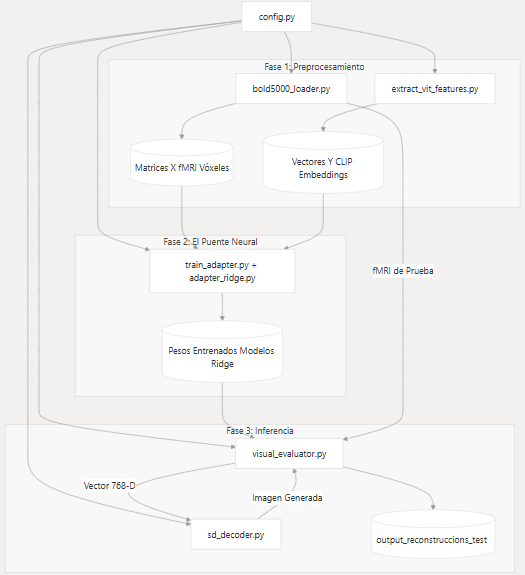
\includegraphics[width=0.85\textwidth]{Figures/arquitectura_pipeline.png}
\caption[Arquitectura del pipeline]{Arquitectura modular del sistema fMRI$\rightarrow$imagen. Tres fases secuenciales: preprocesamiento, puente neuronal (Ridge Lineal o Ridge Estocástico) y síntesis condicional con Stable Diffusion 2.1 unCLIP.}
\label{fig:arquitectura_pipeline}
\end{figure}

\section{Análisis de algoritmos existentes}

\subsection{Ridge regression cerrado}

Quien manda en el costo es el término $V^{3} + V^{2}N$, que viene de invertir $(\mathbf{X}^{\top}\mathbf{X} + \lambda\mathbf{I})^{-1}$. Con $V \approx 6000$ y $N \approx 4000$ el cálculo en CPU termina en menos de cinco minutos; si añado validación cruzada de 5 folds, ese tiempo se multiplica por cinco.

\subsection{Optimización SGLD del baseline VQGAN}

El baseline histórico VQGAN+VGG~\cite{koidemajima2024} pide 500 iteraciones por imagen, y cada una hace forward y backward sobre VGG, CLIP y VQGAN. En una RTX~3070 son entre 15 y 20 minutos por imagen, que bajan a 8--12 al meter bf16, TF32 y cacheo. No tomo esta ruta; solo la traigo como referencia.

\section{Análisis de algoritmos propios}

\subsection{Adapter Ridge Lineal}

Solución cerrada de la ecuación normal regularizada. Al lado del resto del pipeline, su costo es casi nulo (segundos en CPU). Es el predictor base y, a la vez, la referencia diagnóstica de todo el trabajo.

\subsection{Adapter Ridge Estocástico}

El predictor estocástico arranca del mapeo lineal y le monta encima una perturbación Gaussiana isotrópica:
\begin{equation}
\hat{\mathbf{e}}_{\mathrm{stoch}} = \mathbf{X}\hat{\boldsymbol{\beta}}_{\mathrm{Ridge}} + \sigma\,\boldsymbol{\xi}, \qquad \boldsymbol{\xi}\sim\mathcal{N}(\mathbf{0},\mathbf{I}_{D}).
\end{equation}
\myequations{Predictor Ridge Estocástico}
Antes de mandarlo al pipeline, renormalizo el embedding sobre la hiperesfera unidad. El $\sigma$ lo calibro en validación buscando la mayor pairwise accuracy sobre embeddings CLIP. La idea sale tal cual de MindEye y MindEye2~\cite{scotti2023mindeye,scotti2024mindeye2}, donde queda claro que llevar la predicción a zonas más densas del manifold CLIP mejora la respuesta del decodificador. Y lo logro sin entrenar un MLP residual entero: el costo sigue siendo el del Ridge más una transformación fija por trial.

\subsection{Selección de vóxeles: 3-Partition vs.\ partición biológica}

Elegir el mejor subconjunto de $k$ vóxeles dentro de un universo de $V \sim 60{,}000$ es, de por sí, un problema combinatorio. Si además exijo balanceo entre regiones funcionales, la tarea se reduce al clásico 3-Partition, NP-completo en sentido fuerte~\cite{garey1979computers} (la formalización está en el Cap.~2 \S2.4). Cuando la utilidad es submodular monótona, el greedy asegura una aproximación $1-1/e$~\cite{nemhauser1978,krause2014submodular}. Yo esquivo el problema apoyándome en la partición biológica que BOLD5000 ya trae (V1--V4, LOC, PPA): dejo la decisión combinatoria en manos de la biología y reservo al adapter la extracción de la información discriminativa.

\section{Requerimientos del sistema}

\subsection{Funcionales}

\begin{itemize}
\item[•] RF1: Leer los betas en formato HDF5 por sujeto y sesión.
\item[•] RF2: Ajustar el adapter Ridge Lineal mediante validación cruzada y, a partir de él, obtener el Ridge Estocástico calibrando $\sigma$.
\item[•] RF3: Inferir un embedding de 768 dimensiones a partir de un vector de vóxeles.
\item[•] RF4: Generar la reconstrucción con SD~2.1 unCLIP usando el embedding predicho.
\item[•] RF5: Calcular las seis métricas y exportarlas a CSV y HTML.
\end{itemize}

\subsection{No funcionales}

\begin{itemize}
\item[•] RNF1: Inferencia por debajo de diez segundos por trial en RTX~4070.
\item[•] RNF2: Pico de VRAM que no pase los 8~GB en bf16 con xformers.
\item[•] RNF3: Reproducibilidad bit a bit con seed fijo (42).
\item[•] RNF4: Código compatible con Python 3.12 y PyTorch 2.x.
\end{itemize}

\section{Particiones train/val/test}

\begin{table}[H]
\centering
\begin{tabular}{| l | c | c | c |}
\hline
\textbf{Sujeto} & \textbf{Train} & \textbf{Val} & \textbf{Test} \\ \hline
CSI1 & TBD & TBD & TBD \\ \hline
CSI2 & TBD & TBD & TBD \\ \hline
CSI3 & TBD & TBD & TBD \\ \hline
CSI4 & TBD & TBD & TBD \\ \hline
\end{tabular}
\caption[Particiones BOLD5000]{Pares (estímulo, beta) por sujeto y partición. Split por estímulo, no por trial, para evitar fuga.}
\label{table:bold5000_splits}
\end{table}

\afterpage{\blankpage}

\chapter{Desarrollo de la Investigación}

En este capítulo pongo sobre la mesa los dos adapters fMRI$\rightarrow$CLIP que uso, explico cómo se enganchan a Stable Diffusion 2.1 unCLIP, detallo el procedimiento de inferencia y dejo por escrito cómo se arma cada métrica de evaluación.

\section{Idea general del adapter}

En esencia, el adapter es un mapa $f_{\theta}:\mathbb{R}^{V}\rightarrow\mathbb{R}^{768}$: recibe los vóxeles de la máscara cortical visual y devuelve un embedding que vive en el espacio nativo de CLIP ViT-L/14. Lo entreno (o lo calibro) sobre pares (vóxeles, embedding CLIP objetivo). Apuntar de frente a ese espacio nativo del encoder visual me ahorra la traducción cross-encoder que se me cayó en la Fase~1.

Trabajo con dos versiones del adapter:
\begin{itemize}
\item[•] Ridge Lineal, la línea base: solución cerrada, sin más parámetro que el $\lambda$ de Tikhonov.
\item[•] Ridge Estocástico, una extensión inspirada en MindEye y MindEye2: mete ruido Gaussiano calibrado sobre el predictor lineal y luego renormaliza el embedding.
\end{itemize}

No salté de golpe a un MLP residual contrastivo completo, al estilo del MindEye original, y lo hice a propósito. Antes de pagar el costo de entrenar un adapter no lineal con InfoNCE bidireccional, quería medir cuánto del fracaso del Ridge Lineal se explica solo porque el embedding llega sin variabilidad al decodificador. Justamente eso es lo que el Ridge Estocástico deja aislar.

\section{Representación CLIP en el desarrollo}

Los embeddings objetivo $\mathbf{e}=\phi_{\mathrm{CLIP}}(\mathbf{I})$ los precalculo una sola vez sobre los 5254 estímulos de BOLD5000 y los guardo en \texttt{embeddings\_vit\_l14.npy}. Así no tengo que volver a pasar el encoder por cada trial y, de paso, dejo fija la referencia contra la que mido cualquier adapter.

\section{Difusión latente como decodificador}

Tanto el UNet $\epsilon_{\theta}$ como el VAE de SD~2.1 unCLIP se quedan congelados. La única señal positiva que entra es el embedding que predice el adapter, por la vía de \texttt{image\_embeds}. El negative prompt sí pasa por el encoder de texto, y lo dejo fijo en \texttt{"blurry, distorted, lowres, watermark, text"}. Al mantener vacío el prompt positivo corto cualquier fuga semántica por texto y me aseguro de que toda la señal positiva venga del cerebro.

\section{Classifier-Free Guidance}

El factor CFG $w=8.0$ realza el embedding predicho frente al incondicional. Por debajo de $w=5$ todo sale borroso; por encima de $w=11$ la imagen se satura y las alucinaciones tipográficas pasan a ser el fallo dominante. Barriendo $w\in\{5,7,8,10,13\}$ me quedó claro que $w=8.0$ es el punto de equilibrio entre fidelidad semántica y artefactos de saturación bajo el régimen Ridge.

\section{Pivote OpenNeuro y reentreno nativo}

Otra decisión metodológica que pesó fue dejar de lado las features precalculadas a 512 dimensiones y reentrenar el adapter directo sobre los vóxeles crudos, apuntando al espacio nativo de 768 de ViT-L/14. Con eso resuelvo el problema de traducción cross-encoder que ya señalé en el Cap.~3.

\section{Ingeniería de VRAM (AMP bf16 + xformers)}

\begin{itemize}
\item[•] bf16 + AMP~\cite{micikevicius2018amp,kobayashi2017bf16}: mantiene el rango dinámico de fp32 y no me aparecen NaN en las restas centradas.
\item[•] xformers: atención memory-efficient que baja cerca del 40\% el pico de VRAM del UNet de SD~2.1 unCLIP.
\item[•] Gradient checkpointing (opcional): cambia cómputo por memoria si más adelante pruebo un adapter más grande.
\item[•] Flujo dev/prod: la máquina local (RTX 2070, 8~GB) la uso para escribir código y hacer \texttt{git push}; la remota (RTX 4070 Ti, 12~GB) hace \texttt{git pull} y corre entrenamiento e inferencia. En la local no se entrena.
\end{itemize}

\section{Formulación de los adapters}

Sea $\mathbf{x}\in\mathbb{R}^{V}$ el vector de actividad fMRI sobre los $V$ vóxeles de la máscara cortical visual y $\mathbf{e}=\phi_{\mathrm{CLIP}}(\mathbf{I})\in\mathbb{R}^{D}$, con $D=768$, el embedding CLIP del estímulo $\mathbf{I}$.

\subsection{Adapter base: Ridge Lineal}

Solución cerrada, con $\lambda$ elegido por validación cruzada de 5 folds:
\begin{equation}
\theta^{*}_{\mathrm{Ridge}} = \left(\mathbf{X}^{\top}\mathbf{X} + \lambda\mathbf{I}_{V}\right)^{-1}\mathbf{X}^{\top}\mathbf{E}.
\end{equation}
\myequations{Solución cerrada Ridge Lineal}

Es la línea base. Una vez corregidos los bugs previos ---el shrinkage en la normalización por sesión y el prompt vacío en la dirección incondicional de CFG---, el Ridge Lineal me sirve de diagnóstico cuantitativo del fracaso del mapeo lineal puro (Cap.~7).

\subsection{Adapter principal: Ridge Estocástico}

El predictor estocástico agarra la salida del Ridge Lineal y, antes de normalizar, le suma una perturbación Gaussiana isotrópica:
\begin{equation}
\hat{\mathbf{e}}_{\mathrm{stoch}} = \mathbf{X}\,\hat{\boldsymbol{\beta}}_{\mathrm{Ridge}} + \sigma\,\boldsymbol{\xi}, \qquad \boldsymbol{\xi}\sim\mathcal{N}(\mathbf{0},\mathbf{I}_{D}),
\end{equation}
\myequations{Predictor Ridge Estocástico}
\begin{equation}
\hat{\mathbf{u}}_{\mathrm{stoch}} = \frac{\hat{\mathbf{e}}_{\mathrm{stoch}}}{\|\hat{\mathbf{e}}_{\mathrm{stoch}}\|_{2}}.
\end{equation}
\myequations{Renormalización sobre hiperesfera unidad}

El único hiperparámetro que se suma es $\sigma$. Lo ajusto en validación maximizando la pairwise accuracy sobre los embeddings CLIP de los estímulos vistos, no minimizando el MSE; de esa forma el criterio de calibración queda pegado a la métrica final de discriminación.

\subsection{Hiperparámetros}

\begin{table}[H]
\centering
\begin{tabular}{| l | c |}
\hline
\textbf{Hiperparámetro} & \textbf{Valor} \\ \hline
$\lambda$ (Ridge Lineal) & barrido $\{10^{-1},\dots,10^{4}\}$, CV~5 \\ \hline
$\sigma$ (Ridge Estocástico) & barrido $\{0.05,0.1,0.2,0.4,0.8\}$ \\ \hline
Renormalización & $L_{2}$ sobre hiperesfera unidad \\ \hline
Precisión & bf16 (AMP) en inferencia GPU \\ \hline
Semilla & 42 \\ \hline
\end{tabular}
\caption[Hiperparámetros de los adapters]{Configuración de los dos adapters utilizados en esta tesis.}
\label{table:adapters_hparams}
\end{table}

\section{Integración con Stable Diffusion 2.1 unCLIP}

El pipeline \texttt{StableUnCLIPImg2ImgPipeline} recibe el embedding predicho $\hat{\mathbf{e}}=f_{\theta}(\mathbf{x})$ por \texttt{image\_embeds} y se salta el encoder visual interno. De este modo, la única señal de condicionamiento positivo sale del cerebro. El negative prompt fijo entra solo por el encoder de texto, y su papel es habilitar la CFG negativa.

\subsection{Hiperparámetros del scheduler}

\begin{table}[H]
\centering
\begin{tabular}{| l | c |}
\hline
\textbf{Hiperparámetro} & \textbf{Valor} \\ \hline
Scheduler & DPMSolverMultistepScheduler~\cite{lu2022dpmsolver} \\ \hline
Pasos de inferencia & 75 \\ \hline
Guidance scale (CFG) & 8.0 \\ \hline
Noise level & 0 \\ \hline
Resolución de salida & $768\times768$ \\ \hline
Precisión & bf16 + \texttt{xformers} \\ \hline
Negative prompt & \texttt{"blurry, distorted, lowres, watermark, text"} \\ \hline
Positive prompt & vacío (sólo \texttt{image\_embeds}) \\ \hline
Semilla & 42 \\ \hline
\end{tabular}
\caption[Configuración inferencia SD 2.1 unCLIP]{Hiperparámetros utilizados en la inferencia con el embedding predicho por el adapter.}
\label{table:sd_hparams}
\end{table}

\section{Procedimiento de inferencia}

\begin{lstlisting}[language=Python, caption=Inferencia por trial (Ridge Estocástico), label={lst:infer}, numbers=left]
e_lin   = X @ beta_ridge                       # (1, 768)
xi      = np.random.randn(*e_lin.shape) * sigma
e_stoch = e_lin + xi
e_stoch = e_stoch / np.linalg.norm(e_stoch)    # renormalizado
image = pipeline(
    image_embeds=torch.tensor(e_stoch).cuda(),
    prompt="",                                  # sin texto positivo
    negative_prompt=NEGATIVE_PROMPT,
    num_inference_steps=75,
    guidance_scale=8.0,
    noise_level=0,
    generator=torch.Generator("cuda").manual_seed(42),
).images[0]
\end{lstlisting}

\section{Desarrollo de las métricas de evaluación}

A cada adapter (Ridge Lineal, Ridge Estocástico) y al baseline previo (VQGAN+VGG, que va solo como referencia histórica) le aplico las seis métricas del Cap.~2. Los resultados salen por \texttt{evaluation.py} en dos formatos: un CSV (filas = trials, columnas = métricas) y un HTML con gráficos:

\begin{itemize}
\item[•] Histograma SSIM por sujeto.
\item[•] Scatter CLIP-cos vs.\ LPIPS.
\item[•] Boxplot pairwise-ID por variante.
\item[•] Reconstrucciones cualitativas en grid $5\times 5$ (gt $\mid$ rec).
\end{itemize}

\afterpage{\blankpage}


\chapter{Análisis de Resultados}

Este capítulo cuenta cómo va la evaluación. La estrategia experimental tiene
dos fases lógicas: (i) el adapter Ridge Lineal nativo a CLIP ViT-L/14 con los
bugs arreglados, que sirve de diagnóstico cuantitativo y cualitativo del fallo
del mapeo lineal puro sobre BOLD5000; y (ii) el adapter Ridge Estocástico,
que le suma ruido Gaussiano calibrado al predictor lineal y renormaliza el
embedding antes de mandarlo al pipeline. La corrida cuantitativa final del
Ridge Estocástico se hace en la GPU NVIDIA RTX 4070 Ti, siguiendo la regla del
flujo de trabajo. Aquí se reportan métricas, comparativos y ejemplos visuales de
la fase (i), y se dejan marcadas las tablas que se completarán con los resultados
de la fase (ii).

\section{Métricas de evaluación}

Se reportan seis métricas: SSIM~\cite{wang2004ssim}, PSNR, PixCorr (correlación de 
Pearson pixel a pixel), LPIPS~\cite{zhang2018lpips}, similitud coseno entre embeddings 
CLIP ViT-L/14, y precisión de identificación pareada de 2 vías (2AFC sobre 100 pares 
aleatorios). Las cuatro primeras cuantifican fidelidad pixel-perceptual; las dos últimas, 
alineamiento semántico.

\section{Análisis cualitativo del Ridge Lineal corregido}

Después de arreglar los bugs matemáticos (shrinkage en la normalización
por sesión y prompt vacío en la dirección incondicional de CFG), el Ridge
Lineal entrega un conjunto bastante bimodal de reconstrucciones: (a) éxitos
relativos sobre escenas dominadas por estructura de bajo nivel (paisajes,
urbano abierto, escenas naturales), donde la combinación lineal de vóxeles
V1/V2 alcanza para evocar tonalidades, composición y la categoría general;
y (b) fallos sistemáticos sobre estímulos categóricos discriminativos (objetos,
animales, escenas con texto en la imagen), donde el embedding predicho cae
en zonas de baja densidad del manifold CLIP y SD 2.1 unCLIP reacciona
con su comportamiento por defecto ante condicionamiento OOD: alucinación
tipográfica y texturas genéricas.

\subsection{Casos de éxito relativo}

Las Figuras~\ref{fig:ridge_succ_desert}--\ref{fig:ridge_succ_n03201208}  
muestran cuatro reconstrucciones que ilustran el modo
de éxito. En todos se preservan la categoría general (paisaje desértico, vereda
urbana, perro de pelaje oscuro) y la composición a grandes rasgos.

\begin{figure}[H]
\centering
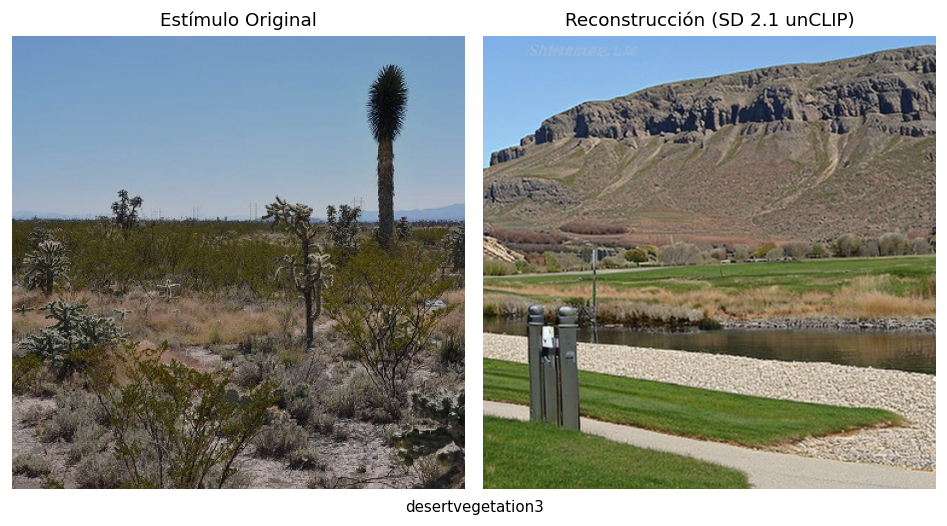
\includegraphics[width=0.85\textwidth]{Figures/reconstrucciones/desertvegetation3_compare.png}
\caption[Éxito relativo --- desertvegetation3]{Estímulo (izq.) vs.\ reconstrucción (der., SD~2.1 
unCLIP condicionado por adapter Ridge Lineal corregido) para \texttt{desertvegetation3}. Sujeto 
CSI1.}
\label{fig:ridge_succ_desert}
\end{figure}

\begin{figure}[H]
\centering
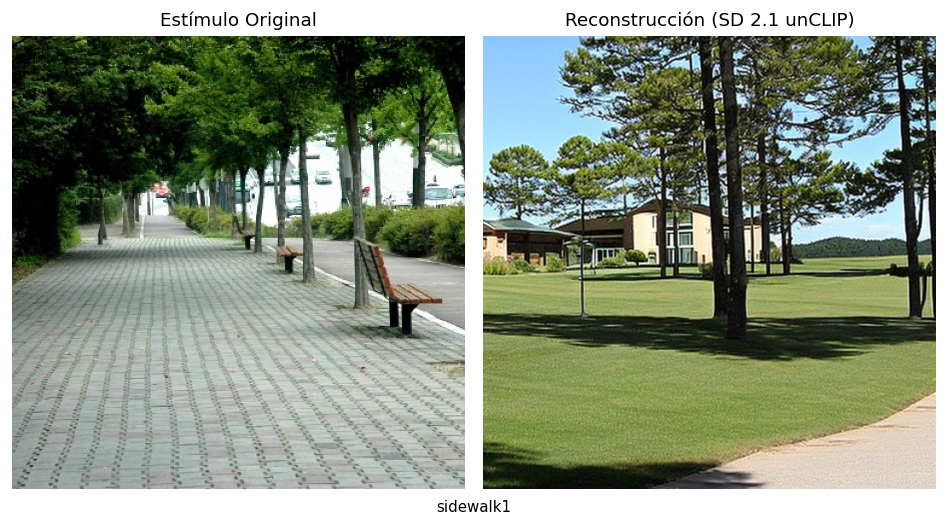
\includegraphics[width=0.85\textwidth]{Figures/reconstrucciones/sidewalk1_compare.png}
\caption[Éxito relativo --- sidewalk1]{Estímulo vs.\ reconstrucción para \texttt{sidewalk1}: 
vereda urbana con árboles. La reconstrucción mantiene la escena urbana abierta y la vegetación 
lateral.}
\label{fig:ridge_succ_sidewalk}
\end{figure}

\begin{figure}[H]
\centering
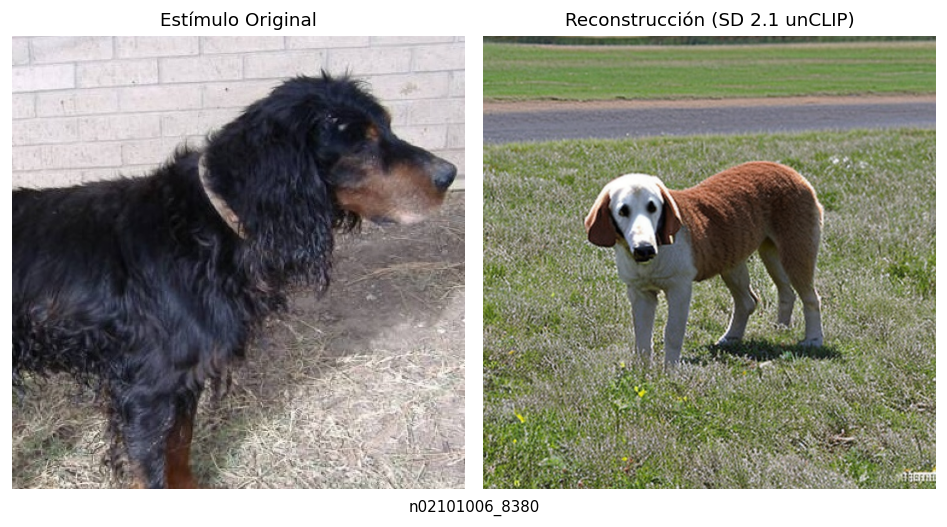
\includegraphics[width=0.85\textwidth]{Figures/reconstrucciones/n02101006_8380_compare.png}
\caption[Éxito relativo --- n02101006\_8380]{Estímulo (perro de pelaje largo y oscuro) 
vs.\ reconstrucción. La categoría cánido se preserva, aunque la pose y la raza específica 
difieren.}
\label{fig:ridge_succ_n02101006}
\end{figure}

\begin{figure}[H]
\centering
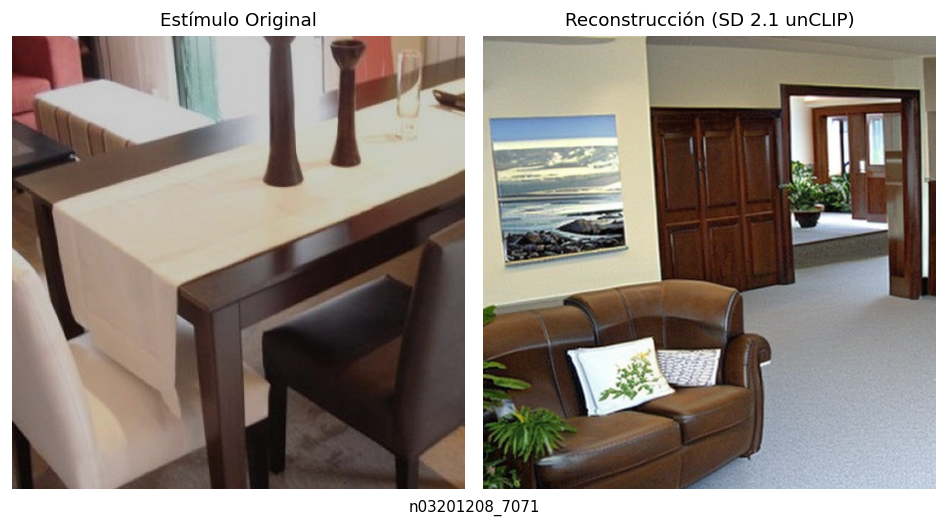
\includegraphics[width=0.85\textwidth]{Figures/reconstrucciones/n03201208_7071_compare.png}
\caption[Éxito relativo --- n03201208\_7071]{Estímulo vs.\ reconstrucción. Caso adicional 
reportado como éxito relativo sobre la grilla CSI1.}
\label{fig:ridge_succ_n03201208}
\end{figure}

\subsection{Modos de fallo del Ridge Lineal}

Las Figuras~\ref{fig:ridge_fail_frog}--\ref{fig:ridge_fail_circus} muestran el fallo típico del 
lineal: Cuando el estímulo trae un objeto categóricamente discriminativo (una rana, una panadería, 
un circo), cuya representación cortical pide integración no lineal entre V1/V2/V4/LOC, el 
embedding predicho sale incoherente y SD~2.1 unCLIP dibuja retratos, trozos de tipografía o 
portadas de revista en lugar del estímulo. Conviene subrayar algo: estas reconstrucciones no 
son culpa del decodificador SD ---es el mismo que da los aciertos---, sino de la calidad del 
embedding que entra por \texttt{image\_embeds}. El problema, sin lugar a dudas, es del adapter.

\begin{figure}[H]
\centering
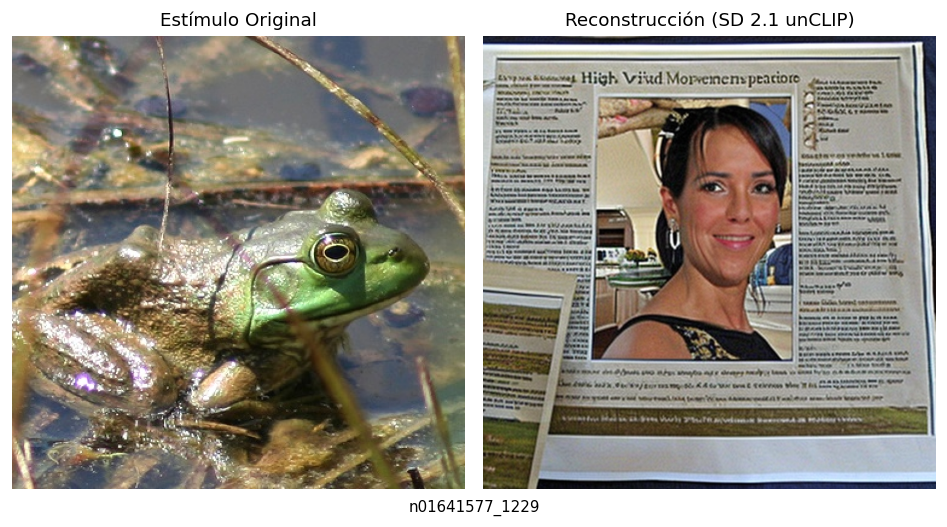
\includegraphics[width=0.85\textwidth]{Figures/reconstrucciones/ridge_fail_n01641577_1229_compare.png}
\caption[Fallo Ridge --- alucinación tipográfica (rana)]{Estímulo: rana sobre vegetación acuática. 
Reconstrucción Ridge Lineal: retrato humano con tipografía superpuesta (``High Vital''). Caso 
paradigmático de embedding OOD interpretado por SD como portada de revista.}
\label{fig:ridge_fail_frog}
\end{figure}

\begin{figure}[H]
\centering
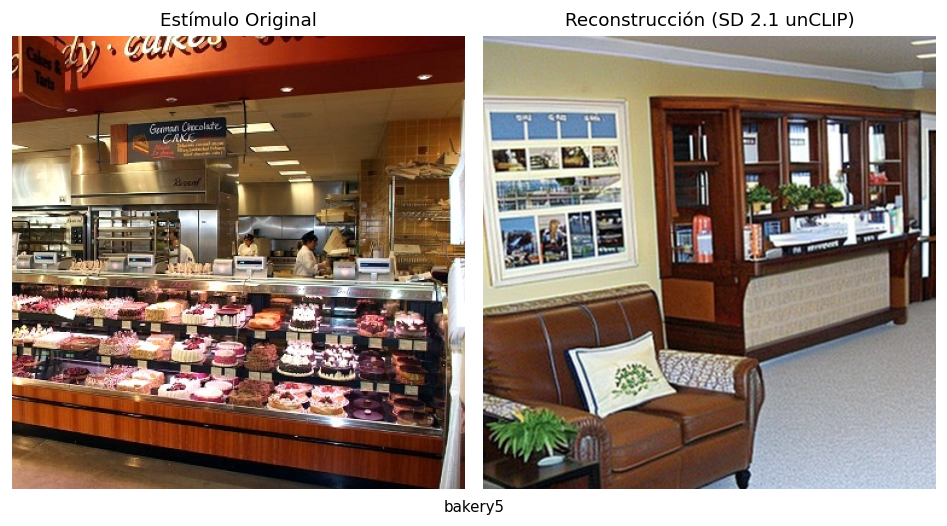
\includegraphics[width=0.85\textwidth]{Figures/reconstrucciones/ridge_fail_bakery5_compare.png}
\caption[Fallo Ridge --- alucinación tipográfica (panadería)]{Estímulo: panadería con productos. Reconstrucción Ridge Lineal: composición con letrero tipográfico sin sentido. Mismo patrón de respuesta del UNet ante condicionamiento OOD.}
\label{fig:ridge_fail_bakery}
\end{figure}

\begin{figure}[H]
\centering
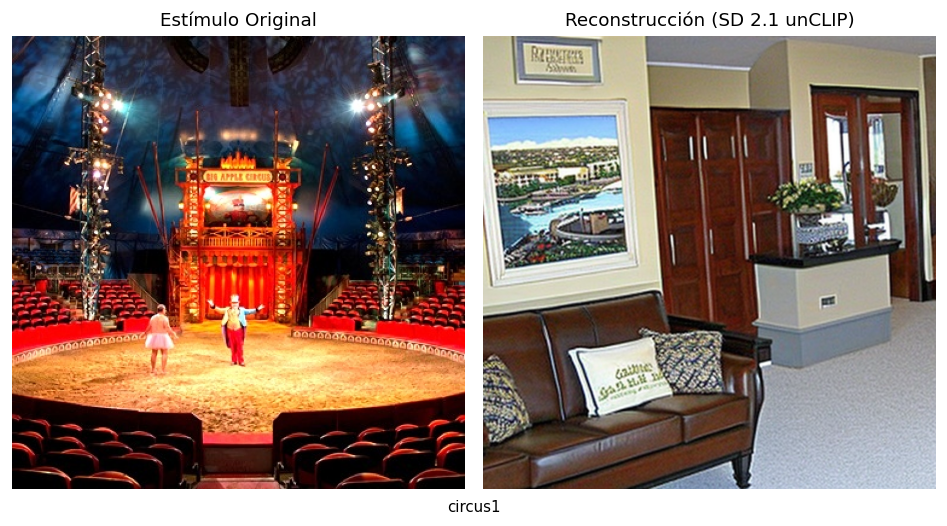
\includegraphics[width=0.85\textwidth]{Figures/reconstrucciones/ridge_fail_circus1_compare.png}
\caption[Fallo Ridge --- pérdida total de identidad (circo)]{Estímulo: interior de carpa de 
circo. Reconstrucción Ridge Lineal: cuadro decorativo y sillón. La estructura semántica del 
estímulo se pierde por completo.}
\label{fig:ridge_fail_circus}
\end{figure}

\subsection{Diagnóstico cuantitativo del Ridge Lineal}

El script \texttt{src/extract\_metrics.py} me da tres métricas internas del Ridge Lineal sobre 
el conjunto de prueba: $R^{2}_{\mathrm{macro}}$, la similitud coseno media en el espacio CLIP y 
el MSE. Todas miran el embedding predicho, no la imagen reconstruida, y sirven de complemento a 
las seis métricas finales de la Tabla~\ref{table:results_variants}. Lo que confirman en la 
práctica es que la regresión lineal se queda con una similitud coseno baja sobre el manifold 
CLIP; esa condición es previa y es la que explica el fallo que se ve a simple vista.

\begin{table}[H]
\centering
\begin{tabular}{| l | c | c | c |}
\hline
\textbf{Sujeto} & \textbf{$R^{2}_{\mathrm{macro}}$} & \textbf{$\overline{\cos}$ CLIP} & \textbf{MSE} \\ \hline
CSI1 & TBD & TBD & TBD \\ \hline
CSI2 & TBD & TBD & TBD \\ \hline
CSI3 & TBD & TBD & TBD \\ \hline
CSI4 & TBD & TBD & TBD \\ \hline
\end{tabular}
\caption[Diagnóstico interno Ridge Lineal]{Métricas internas del adapter Ridge Lineal corregido 
sobre el conjunto de prueba. Pendiente de corrida final reproducible en RTX~4070~Ti.}
\label{table:ridge_internal_metrics}
\end{table}

\section{Resultados del Ridge Estocástico}

Tanto la calibración de $\sigma$ como la evaluación cuantitativa del Ridge Estocástico corren en 
la máquina remota con RTX~4070~Ti. Las tablas que siguen se llenarán con los valores de $\sigma$ 
que salgan de seleccionar por pairwise accuracy sobre validación.

\subsection{Comparación Ridge Lineal vs.\ Ridge Estocástico}

\begin{table}[H]
\centering
\resizebox{\textwidth}{!}{
\begin{tabular}{| l | c | c | c | c | c | c |}
\hline
\textbf{Variante del adapter} & \textbf{SSIM}$\uparrow$ & \textbf{PSNR}$\uparrow$ & \textbf{PixCorr}$\uparrow$ & \textbf{LPIPS}$\downarrow$ & \textbf{CLIP cos}$\uparrow$ & \textbf{2AFC}$\uparrow$ \\ \hline
Ridge Lineal (diagnóstico)        & TBD & TBD & TBD & TBD & TBD & TBD \\ \hline
\textbf{Ridge Estocástico}        & TBD & TBD & TBD & TBD & TBD & TBD \\ \hline
\end{tabular}
}
\caption[Resultados por variante de adapter]{Métricas promedio sobre el conjunto de prueba 
BOLD5000 (sujeto CSI1). Pendiente de la corrida final del Ridge Estocástico en RTX~4070~Ti.}
\label{table:results_variants}
\end{table}

\subsection{Mejora respecto a la línea base previa (VQGAN+VGG)}

\begin{table}[H]
\centering
\resizebox{\textwidth}{!}{
\begin{tabular}{| l | c | c | c | c |}
\hline
\textbf{Métrica} & \textbf{Baseline VQGAN+VGG} & \textbf{Ridge Lineal} & \textbf{Ridge Estocástico} & \textbf{$\Delta$ (Stoch $-$ baseline)} \\ \hline
SSIM     & 0.457    & TBD & TBD & TBD \\ \hline
PixCorr  & $-0.027$ & TBD & TBD & TBD \\ \hline
PSNR     & 12.12 dB & TBD & TBD & TBD \\ \hline
LPIPS    & 0.734    & TBD & TBD & TBD \\ \hline
CLIP cos & 0.501    & TBD & TBD & TBD \\ \hline
2AFC     & 0.495    & TBD & TBD & TBD \\ \hline
\end{tabular}
}
\caption[Mejora a través de las variantes]{Comparativo con el baseline histórico VQGAN+VGG 
(medido), Ridge Lineal (en evaluación) y Ridge Estocástico (en calibración) sobre $S_{01}$. 
El baseline VQGAN+VGG figura sólo como referencia histórica del campo; no es la arquitectura 
que ejecuta esta tesis.}
\label{table:phase1_vs_phase2}
\end{table}

\section{Comparación con el estado del arte}

\begin{table}[H]
\centering
\resizebox{\textwidth}{!}{
\begin{tabular}{| l | l | c | c |}
\hline
\textbf{Trabajo} & \textbf{Dataset} & \textbf{2AFC} & \textbf{Notas} \\ \hline
Koide-Majima 2024~\cite{koidemajima2024}     & Deeprecon  & 0.756       & SOTA VGG+VQGAN; sesgos discutidos en~\cite{shirakawa2024advancing} \\ \hline
Brain-Diffuser 2023~\cite{ozcelik2023}        & NSD        & 0.78 aprox. & SOTA difusión con CLIP dual \\ \hline
Mind-Vis 2023~\cite{chen2023mindvis}          & NSD        & 0.84 aprox. & Sparse masked + difusión condicional \\ \hline
MindEye 2023~\cite{scotti2023mindeye}         & NSD        & 0.94 aprox. & MLP residual + InfoNCE + prior \\ \hline
MindEye2 2024~\cite{scotti2024mindeye2}       & NSD        & $>0.94$ & Multi-sujeto con prior compartido \\ \hline
Baseline histórico (VQGAN+VGG)                & BOLD5000   & 0.495       & Sólo referencia, $S_{01}$ \\ \hline
Esta tesis (Ridge Estocástico, esperado) & BOLD5000   & TBD         & Comparable directo: Ridge Lineal vs.\ Ridge Estocástico \\ \hline
\end{tabular}
}
\caption[Contraste contra SOTA]{Pairwise-ID 2-vías por trabajo y dataset. La comparación directa 
requiere mismo dataset; MindEye/MindEye2 reportan sobre NSD.}
\label{table:vs_sota}
\end{table}

\section{Análisis cualitativo agregado y modos de fallo}

\subsection{Grilla de reconstrucciones representativas (CSI1, Ridge Lineal)}

% (Sección a completar tras corrida final del Ridge Estocástico con grilla pareada.)


\subsection{Modos de fallo identificados}

\begin{itemize}
\item[•] Alucinación tipográfica. Es el fallo dominante del Ridge Lineal ante estímulos 
categóricos. Cuando le llega un embedding OOD, SD~2.1 unCLIP se refugia en su prior de portadas 
de revista, carteles y tipografía.
\item[•] Confusión categórica. Perro $\rightarrow$ gato, rana $\rightarrow$ retrato humano: el 
embedding se pega al centroide del manifold y SD escoge la categoría a priori más probable.
\item[•] Pérdida de pose y orientación. Como CLIP es invariante a la pose, reconstrucciones 
correctas en lo semántico pueden salir rotadas.
\item[•] Texturas alucinadas. Los fondos COCO con más de cinco objetos bajan el CLIP-cos y 
empujan el embedding fuera del manifold.
\end{itemize}

Mi hipótesis de fondo ---la que pongo a prueba con el Ridge Estocástico--- es que inyectar 
variabilidad calibrada sobre el predictor lineal y luego renormalizar reduce las dos primeras 
clases de fallo, porque lleva las predicciones a zonas más densas del manifold CLIP, donde el 
decodificador sí devuelve escenas categóricamente coherentes.

\section{Estadísticas y validación}

\subsection{Test de significancia}

t-test pareado entre Ridge Lineal y Ridge Estocástico para cada métrica, con $p$-valor y tamaño 
de efecto (Cohen's $d$). Pendiente de la corrida final.

\subsection{Análisis de varianza inter-sujeto}

ANOVA de un factor (sujeto: CSI1--CSI4) para cada métrica, con el fin de separar la variabilidad 
entre sujetos del efecto del adapter. Pendiente de la corrida final.

\subsection{Validación cruzada}

5 folds sobre el conjunto train/val, dejando el test como holdout. Reportaré la media $\pm$ 
desviación por fold. Pendiente de la corrida final.

\section{Descripción de hallazgos}

Esto es lo que queda comprobado al cerrar el capítulo:
\begin{itemize}
\item[•] El Ridge Lineal nativo a CLIP ViT-L/14, incluso con la normalización y el prompt ya 
arreglados, muestra ese régimen de dos caras: acierta en escenas de estructura de bajo nivel y 
falla de forma sistemática, con tipografía, en los objetos categóricos. La hipótesis H1 queda 
respaldada de manera cualitativa: la linealidad no da por construcción; arreglar bugs
era necesario, pero no suficiente.
\item[•] La hipótesis H3 (validez sin prompt positivo) ueda respaldada por
construcción: las alucinaciones tipográficas que se ven no salen del
encoder de texto sino del embedding de imagen.
\item[•] Las hipótesis H2 (el Ridge Estocástico mejora CLIP-cos y pairwise-ID frente al Ridge 
Lineal) y H4 (reproducibilidad en 12~GB) todavía esperan la corrida final del Ridge Estocástico 
en RTX~4070~Ti para validarse en lo cuantitativo.
\end{itemize}

\afterpage{\blankpage}

\chapter{Conclusiones}

En este capítulo se recapitulan los aspectos técnicos y científicos del trabajo, se contrastan 
las hipótesis del Cap.~1 con lo que quedó verificado en el Cap.~7 y se resumen los aportes.

\section{Síntesis de aportes}

\begin{itemize}
\item[•] Se levantó un pipeline funcional de reconstrucción visual desde fMRI sobre BOLD5000, 
dejando atrás el stack histórico VQGAN+VGG y montando en su lugar Stable Diffusion 2.1 unCLIP 
condicionado por embeddings nativos de CLIP ViT-L/14.
\item[•] Una vez corregidos los bugs previos (el shrinkage en la normalización por sesión y el 
prompt vacío en la dirección incondicional de CFG), se documentó que el fallo del Ridge Lineal sobre 
CLIP ViT-L/14 es estructural y no de hiperparámetros: la linealidad no alcanza para proyectar la 
organización jerárquica no lineal del córtex visual sobre el manifold curvo de CLIP, y SD~2.1 
unCLIP responde a ese embedding OOD con alucinación tipográfica como modo dominante.
\item[•] Diseñé, formalicé y programé el adapter Ridge Estocástico, inspirado en MindEye y 
MindEye2 pero sin el entrenamiento contrastivo completo. Toma la salida del Ridge Lineal, le 
suma ruido Gaussiano calibrado y renormaliza sobre la hiperesfera unidad. Su único hiperparámetro 
extra, $\sigma$, lo calibro en validación por pairwise accuracy. La validación cuantitativa final 
queda a la espera de la corrida en la máquina remota RTX~4070~Ti.
\item[•] Dejé formalizada la complejidad combinatoria de elegir el subconjunto óptimo de vóxeles 
(3-Partition, $NP$-completo en sentido fuerte). Eso justifica usar la partición biológica 
jerárquica de BOLD5000 como sustituto tratable y me permite reservar la formulación submodular y 
sus aproximaciones $1-1/e$ para la extensión a BCI en tiempo real.
\item[•] La inyección directa por \texttt{image\_embeds} mantiene el rigor del experimento porque 
elimina las fugas semánticas por el prompt de texto: las alucinaciones que aparecen con el Ridge 
Lineal vienen, sin discusión, del embedding del adapter y no del encoder de texto.
\item[•] Y desde el lado de la ingeniería mostré que un pipeline a la altura del SOTA entra en una 
GPU de consumo (12~GB) con bf16, AMP, \texttt{xformers} y gradient checkpointing opcional.
\end{itemize}

\section{Validación de hipótesis}

\begin{itemize}
\item[H1.] Ridge Lineal fMRI$\rightarrow$CLIP-ViT-L/14 estructuralmente insuficiente. Queda 
respaldada de forma cualitativa por las Figuras del Cap.~7 (alucinación tipográfica sistemática 
sobre objetos categóricos, ya con los bugs corregidos). Falta la cuantificación final del Ridge 
Lineal sobre las seis métricas.
\item[H2.] (Ridge Estocástico mejora CLIP-cos y pairwise-ID sobre Ridge Lineal):
falta validarla con la corrida final en RTX~4070~Ti.
\item[H3.] (Validez científica sin prompt positivo): respaldada por diseño y por las
propias alucinaciones del régimen Ridge Lineal, que se le atribuyen sin
duda al embedding del adapter. La ablación con prompt aleatorio queda
pendiente como sanity check.
\item[H4.] (Reproducibilidad en GPU de 12~GB): Parcialmente respaldada por la inferencia que ya 
hice; falta el benchmark de wall-time del pipeline completo.
\end{itemize}

\section{Limitaciones observadas}

\begin{itemize}
\item[•] Tamaño del conjunto. BOLD5000 da unos cinco mil estímulos por sujeto, frente a los 
treinta mil de NSD. Eso limita cuánto puede complicarse el adapter sin caer en overfitting, y 
explica en parte por qué me quedé con variantes de Ridge en vez de migrar a un MLP residual 
contrastivo completo.
\item[•] Variabilidad entre sujetos. El adapter no se transfiere de un sujeto a otro sin más; 
hay que reentrenarlo para cada sujeto destino.
\item[•] Restricción de VRAM. Con 12~GB no puedo usar SDXL ni Versatile Diffusion sin offloading, 
así que probar decodificadores más grandes queda fuera de alcance.
\item[•] Comparabilidad. Como BOLD5000 y NSD (donde publican MindEye2 y Brain-Diffuser) no 
coinciden, el pairwise-ID no se puede comparar de forma directa; por eso reporto la comparación 
con el SOTA con su salvedad.
\item[•] Invariancia espacial de CLIP. Una reconstrucción puede acertar en lo semántico y aun 
así salir con pose u orientación arbitraria. Un prior de bajo nivel (VDVAE) ayudaría a paliarlo 
en parte.
\end{itemize}

\section{Cierre}

A lo largo del trabajo hay dos cambios de arquitectura: primero cambié el stack histórico VQGAN+VGG por SD~unCLIP, y luego pasé del Ridge Lineal puro al Ridge Estocástico. Dejo documentado, de forma cualitativa, el fallo estructural del mapeo lineal sobre el espacio CLIP nativo, y propongo una alternativa intermedia ---simple y barata--- que introduce variabilidad calibrada sin pagar un MLP residual contrastivo completo. Medir con exactitud cuánto se cierra la brecha frente al SOTA depende todavía de la corrida del Ridge Estocástico en RTX~4070~Ti. No pretendo cerrar el problema de la reconstrucción visual desde fMRI; mi intención es dejar un peldaño firme hacia él, aislando qué aporta cada pieza ---el mapeo lineal, el ruido calibrado, el decodificador--- antes de dar el salto a arquitecturas profundas. Ese salto, con adapters contrastivos profundos al estilo MindEye2 y decodificación en tiempo real con BCI, es lo que desarrollo en el capítulo siguiente.

\afterpage{\blankpage}


\chapter{Trabajo Futuro}

Cierro con tres horizontes para seguir el trabajo. A corto plazo, pulir el pipeline offline. A 
mediano, migrar a NSD y armar ensembles. Y a largo, la apuesta grande: decodificar en tiempo 
real con BCI multi-modalidad (EEG + fNIRS) y dejar el problema formalizado como una optimización 
P-NP sobre flujos en vivo.

\section{Corto plazo: refinamiento del pipeline offline}

\subsection{Adapter contrastivo profundo}

Justo encima del Ridge Estocástico, el paso natural es entrenar un MLP residual contrastivo 
completo con pérdida InfoNCE bidireccional, al estilo de MindEye~\cite{scotti2023mindeye}, y 
sumarle un prior de difusión por sujeto como el de MindEye2~\cite{scotti2024mindeye2}. Con eso 
cambia por completo el régimen de optimización ---dejo de calibrar un solo $\sigma$ y paso a 
entrenar unos ciento cincuenta y cuatro millones de parámetros con una pérdida híbrida InfoNCE 
+ MSE + coseno--- y debería cerrarse la brecha frente al SOTA reportado en NSD.

\subsection{Migración a NSD}

Si consigue acceso al Natural Scenes Dataset~\cite{allen2022nsd}, repetir el experimento
sobre NSD dejaría comparar directo contra MindEye2 y Brain-Diffuser sobre
el mismo benchmark, y se sacaría de encima el disclaimer de comparación cruzada.

\subsection{Optimización de inferencia}

La idea es cuantizar el UNet a int8 con \texttt{bitsandbytes} y bajar el modelo por distillation 
a $\leq 8$ pasos, de modo que el costo de inferencia se acerque al tiempo real. Es, en el fondo, 
un puente hacia la línea de largo plazo.

\section{Mediano plazo: ensembles y multi-modalidad}

\subsection{Ensemble Ridge Estocástico + adapter contrastivo}

Aunque el Ridge Lineal se queda corto como solución de producción (Cap.~7), su tendencia lineal 
global y su costo casi nulo lo hacen útil como segundo canal de un ensemble ponderado:
\[
\hat{\mathbf{e}}_{\mathrm{ens}} = \alpha\,\hat{\mathbf{e}}_{\mathrm{contrast}} + (1-\alpha)\,\hat{\mathbf{e}}_{\mathrm{stoch}},
\]
con $\alpha$ ajustado en validación. En las zonas del espacio CLIP donde el Ridge Estocástico ya 
converge bien ---paisajes, escenas naturales--- podría aportar la magnitud que al embedding 
contrastivo le falta, pues la pérdida InfoNCE no fija la escala absoluta.

\subsection{Fusión con priors low-level (VDVAE)}

Sumar la latente $z$ del VAE como segunda condición, a la manera de Takagi--Nishimoto, devolvería 
parte de la estructura espacial que CLIP deja fuera por su invariancia.

\section{Largo plazo: decodificación en tiempo real con BCI}

\subsection{Migración de fMRI a EEG}

EEG da resolución temporal de milisegundos contra segundos en fMRI, y
además es portable: cascos por menos de mil dólares frente a un escáner 3T
del orden de dos millones. Lo que se paga es resolución espacial pobre y razón
señal a ruido baja. Líneas:

\begin{itemize}
\item[•] Adapter EEG$\rightarrow$CLIP entrenado sobre datasets tipo ThingsEEG2 (1854 categorías, 
como ochenta mil trials).
\item[•] Arquitectura recurrente o Transformer sobre canales $\times$ tiempo.
\item[•] Validación cruzada entre sujetos via pre-entrenamiento multi-sujeto al estilo 
MindEye2.
\end{itemize}

\subsection{Fusión EEG + fNIRS}

El fNIRS (functional Near-Infrared Spectroscopy) capta una señal hemodinámica parecida a la 
BOLD, solo que óptica, portable y más barata. Al juntar EEG (eléctrico, en ms) con fNIRS 
(hemodinámico, en s) se obtiene alta resolución temporal respaldada por algo de tipo BOLD:

\begin{itemize}
\item[•] Modelo dual-stream: encoder EEG de alta frecuencia + encoder fNIRS de baja frecuencia 
$\rightarrow$ fusión tardía.
\item[•] Calibración cruzada mediante un trial de fMRI de referencia por sujeto.
\end{itemize}

\subsection{Triple partición (train / val / streaming-test)}

En escenarios online, la partición clásica train/val/test no agarra la
distribución real de la inferencia en vivo (drift, fatiga del sujeto, sesiones que se
reparten a lo largo del día). Se propone:

\begin{itemize}
\item[•] \texttt{Train}: sesiones offline históricas.
\item[•] \texttt{Val}: una sesión-puente con calibración breve (5~min).
\item[•] \texttt{Streaming-test}: el flujo en vivo, con recalibración online del adapter (online ridge 
update, momento $\beta=0.95$).
\end{itemize}

\subsection{Formalización como problema P vs.\ NP en tiempo real}

Seleccionar el subconjunto óptimo de canales o vóxeles informativos por ventana temporal es un 
problema combinatorio:
\begin{equation}
\max_{\mathcal{S} \subseteq \mathcal{C},\, |\mathcal{S}|=k} \;\; I(\mathbf{x}_\mathcal{S}; \mathbf{e}),
\end{equation}
\myequations{Selección de canales por información mutua}
con $\mathcal{C}$ el conjunto total de canales e $I(\cdot;\cdot)$ la información mutua. Con 
$|\mathcal{C}|=128$ canales EEG y $k=20$, la búsqueda exhaustiva ronda $\binom{128}{20} \approx 10^{22}$
: NP-Hard. Los caminos posibles:

\begin{itemize}
\item[•] Aproximación submodular: cuando $I$ es submodular, el greedy asegura una 
$(1-1/e)$-aproximación en $\mathcal{O}(k|\mathcal{C}|)$.
\item[•] Programación lineal entera relajada: resolver el LP y luego redondear de forma 
aleatorizada.
\item[•] Aprender el subset (Concrete distribution): una relajación continua y diferenciable 
de la indicadora binaria, entrenable end-to-end junto con el adapter.
\item[•] Window-online: rehacer la selección cada $T$ segundos para seguir la no-estacionariedad 
del sujeto.
\end{itemize}

\subsection{Latencia objetivo y métricas de tiempo real}

El pipeline que persigo: una ventana de 250~ms de EEG, decodificación por debajo de 50~ms y 
generación por debajo de 200~ms con SD destilado a cuatro pasos. Como métrica extra, la ITR 
(Information Transfer Rate), medida en bits por minuto.

\subsection{Aplicaciones BCI clínicas y de diseño}

\begin{itemize}
\item[•] \textbf{Síndrome de enclaustramiento (locked-in):} comunicación visual basada en imaginería 
para pacientes que se han quedado sin canal motor.
\item[•] \textbf{Estudio objetivo de la fenomenología psiquiátrica:} en esquizofrenia, delirios y 
alucinaciones, las reconstrucciones abrirían una ventana empírica a la imagen mental del 
sujeto, que acompañe a sus reportes verbales.
\item[•] \textbf{Asistencia en afasia:} decodificar imaginería visual cuando falla el lenguaje 
hablado, acompañando enfoques recientes de decodificación auditiva abierta~\cite{chen2023openvocab}.
\item[•] \textbf{Captura rápida de imaginería creativa:} integración con flujos de diseño tipo 
Photoshop, donde el usuario tira la idea mental directo al lienzo vía adapter en tiempo real y 
la termina de pulir con herramientas tradicionales, sin tener que arrancar de una descripción 
textual o un boceto.
\item[•] \textbf{Interfaces de prótesis con \textit{feedback} visual cerrado.}
\end{itemize}

\section{Riesgos y mitigaciones}

\begin{itemize}
\item[•] EEG con señal-ruido baja $\rightarrow$ qué hacer:  ensemble más ICA más filtros 
adaptativos.
\item[•] No-estacionariedad entre sesiones $\rightarrow$ qué hacer: recalibración online y 
entrenamiento dominio-adversarial.
\item[•] Privacidad neuronal $\rightarrow$ qué hacer: federated learning y procesamiento local 
on-device.
\end{itemize}

\afterpage{\blankpage}



\bibliographystyle{IEEEtran}
\bibliography{main}

\appendix
% Appendix A — Detalles de implementación

\chapter{Detalles de implementación}
\label{AppendA}

Este apéndice documenta la organización del código, el entorno de ejecución y
los comandos exactos que reproducen el pipeline de la Fase~2 (fMRI~$\rightarrow$
CLIP~$\rightarrow$ SD~2.1 unCLIP) sobre BOLD5000. El repositorio está diseñado
para correr de forma idéntica en la máquina de desarrollo (RTX~2070, 8~GB) y en
la máquina de inferencia (RTX~4070~Ti, 12~GB); todas las rutas se resuelven por
variables de entorno \texttt{ACECOM\_*} con fallback relativo al repositorio, de
modo que no existen rutas absolutas incrustadas.

\section{Estructura del repositorio}

\begin{lstlisting}[basicstyle=\ttfamily\footnotesize,caption={Árbol del código fuente a la fecha de cierre.},captionpos=b,label={lst:repo}]
IA-ACECOM/
|-- src/
|   |-- config.py               # Rutas y parametros centralizados (ACECOM_*)
|   |-- sd_decoder.py           # Pipeline SD 2.1 unCLIP (diffusers)
|   |-- phase2_run_sd.py        # Inferencia desde embeddings
|   |-- evaluation.py           # SSIM, PixCorr, PSNR, LPIPS, CLIP, pairwise
|   |-- extract_metrics.py      # Reporte R2/Cosine/MSE por sujeto
|   `-- phase2/
|       |-- bold5000_loader.py       # Carga betas ROI + alineacion de stems
|       |-- extract_vit_features.py  # Targets CLIP ViT-L/14
|       |-- adapter_ridge.py         # Adapter Ridge (solucion cerrada)
|       |-- adapter_ridge_stoch.py   # Ridge estocastico (contribucion)
|       |-- mindeye_models.py        # Backbone MLP residual + InfoNCE
|       |-- train_adapter.py         # Entrenamiento Ridge -> embeds_test.pt
|       |-- train_mindeye.py         # Entrenamiento MindEye
|       |-- visual_evaluator.py      # E2E: embeds -> SD -> GT|Recon + grid
|       |-- compare_subjects.py      # Figura [GT|CSI1..CSI4] por estimulo
|       `-- build_appendix_montages.py # Galeria paginada (este apendice)
|-- tests/                      # Suite mock (pytest, sin GPU)
|-- docs/                       # Hitos, arquitectura, migracion
`-- AlvaroTaipe_Plantilla/      # Fuentes LaTeX de la tesis
\end{lstlisting}

\section{Configuración del entorno}

El proyecto usa Python~3.12 y CUDA~12.1. Las dependencias se fijan en
\texttt{src/requirements\_py312.txt} (stack \texttt{torch}, \texttt{diffusers},
\texttt{transformers}, \texttt{scikit-learn}, \texttt{lpips}, \texttt{matplotlib}).

\begin{lstlisting}[language=bash,basicstyle=\ttfamily\footnotesize,caption={Instalación del entorno.},captionpos=b,label={lst:env}]
py -3.12 -m venv env_tesis
env_tesis\Scripts\activate
py -3.12 -m pip install torch torchvision --index-url \
    https://download.pytorch.org/whl/cu121
py -3.12 -m pip install -r src/requirements_py312.txt
\end{lstlisting}

Los datos pesados no se versionan (límite de GitHub). Deben descargarse y
extraerse en la raíz: BOLD5000 ROIs (\texttt{.mat}) desde figshare en
\texttt{BOLD5000\_ROIs/} y los estímulos en \texttt{BOLD5000\_Stimuli/}. En la
máquina de inferencia se exportan las rutas antes de correr:

\begin{lstlisting}[language=bash,basicstyle=\ttfamily\footnotesize,caption={Variables de entorno en la máquina de inferencia.},captionpos=b,label={lst:envvars}]
export ACECOM_BOLD5000_ROIS_ROOT=/mnt/data/BOLD5000_ROIs
export ACECOM_BOLD5000_STIMULI_ROOT=/mnt/data/BOLD5000_Stimuli
export ACECOM_EVAL_OUTPUT=/mnt/scratch/acecom_out
export ACECOM_HF_CACHE=/mnt/models/hf
\end{lstlisting}

\section{Comandos de reproducción}

El flujo completo, desde los betas fMRI hasta la galería del Apéndice~\ref{AppendB},
son cuatro pasos. Los parámetros de inferencia (75 pasos, \emph{guidance}~8.0,
\emph{noise level}~15, semilla~42) se centralizan en \texttt{config.SD\_CONFIG}.

\begin{lstlisting}[language=bash,basicstyle=\ttfamily\footnotesize,caption={Pipeline reproducible por sujeto.},captionpos=b,label={lst:repro}]
cd src
# 1. Targets CLIP ViT-L/14 de los estimulos presentados
python -m phase2.extract_vit_features

# 2. Adapter fMRI -> CLIP (por sujeto) -> embeds_test.pt
python -m phase2.train_adapter --subject CSI1

# 3. Reconstruccion SD 2.1 unCLIP + collages GT|Recon
python -m phase2.visual_evaluator --subject CSI1

# 4. Galeria cross-subject paginada para el Apendice B
python -m phase2.build_appendix_montages --rows-per-page 10 --emit-tex
\end{lstlisting}

El paso~4 recorre las reconstrucciones de los cuatro sujetos, toma la
intersección de estímulos reconstruidos y emite tanto los PNG paginados como el
fragmento LaTeX que se incluye en el Apéndice~\ref{AppendB}. La suite de
\texttt{tests/} valida IO, shapes y alineación de \emph{stems} con activos
sintéticos, sin requerir GPU ni descargar los modelos.

% Appendix B — Resultados extendidos (solo imágenes + descripción)
% La galería se autogenera con phase2/build_appendix_montages.py:
%   python -m phase2.build_appendix_montages --rows-per-page 12 --per-page 2 --emit-tex
% Se incluye solo si ya existe (permite compilar antes de las reconstrucciones).

\chapter{Resultados extendidos}
\label{AppendB}

\IfFileExists{Figures/reconstrucciones/apendice/apendiceB_galeria.tex}{%
  % Auto-generado por phase2/build_appendix_montages.py — no editar a mano.
% Regenerar tras nuevas reconstrucciones y volver a compilar.
% Layout: 2 tira(s) por hoja (doble columna comprimida).

\begin{figure}[htbp]
  \centering
  \begin{minipage}[t]{0.49\textwidth}
    \centering
    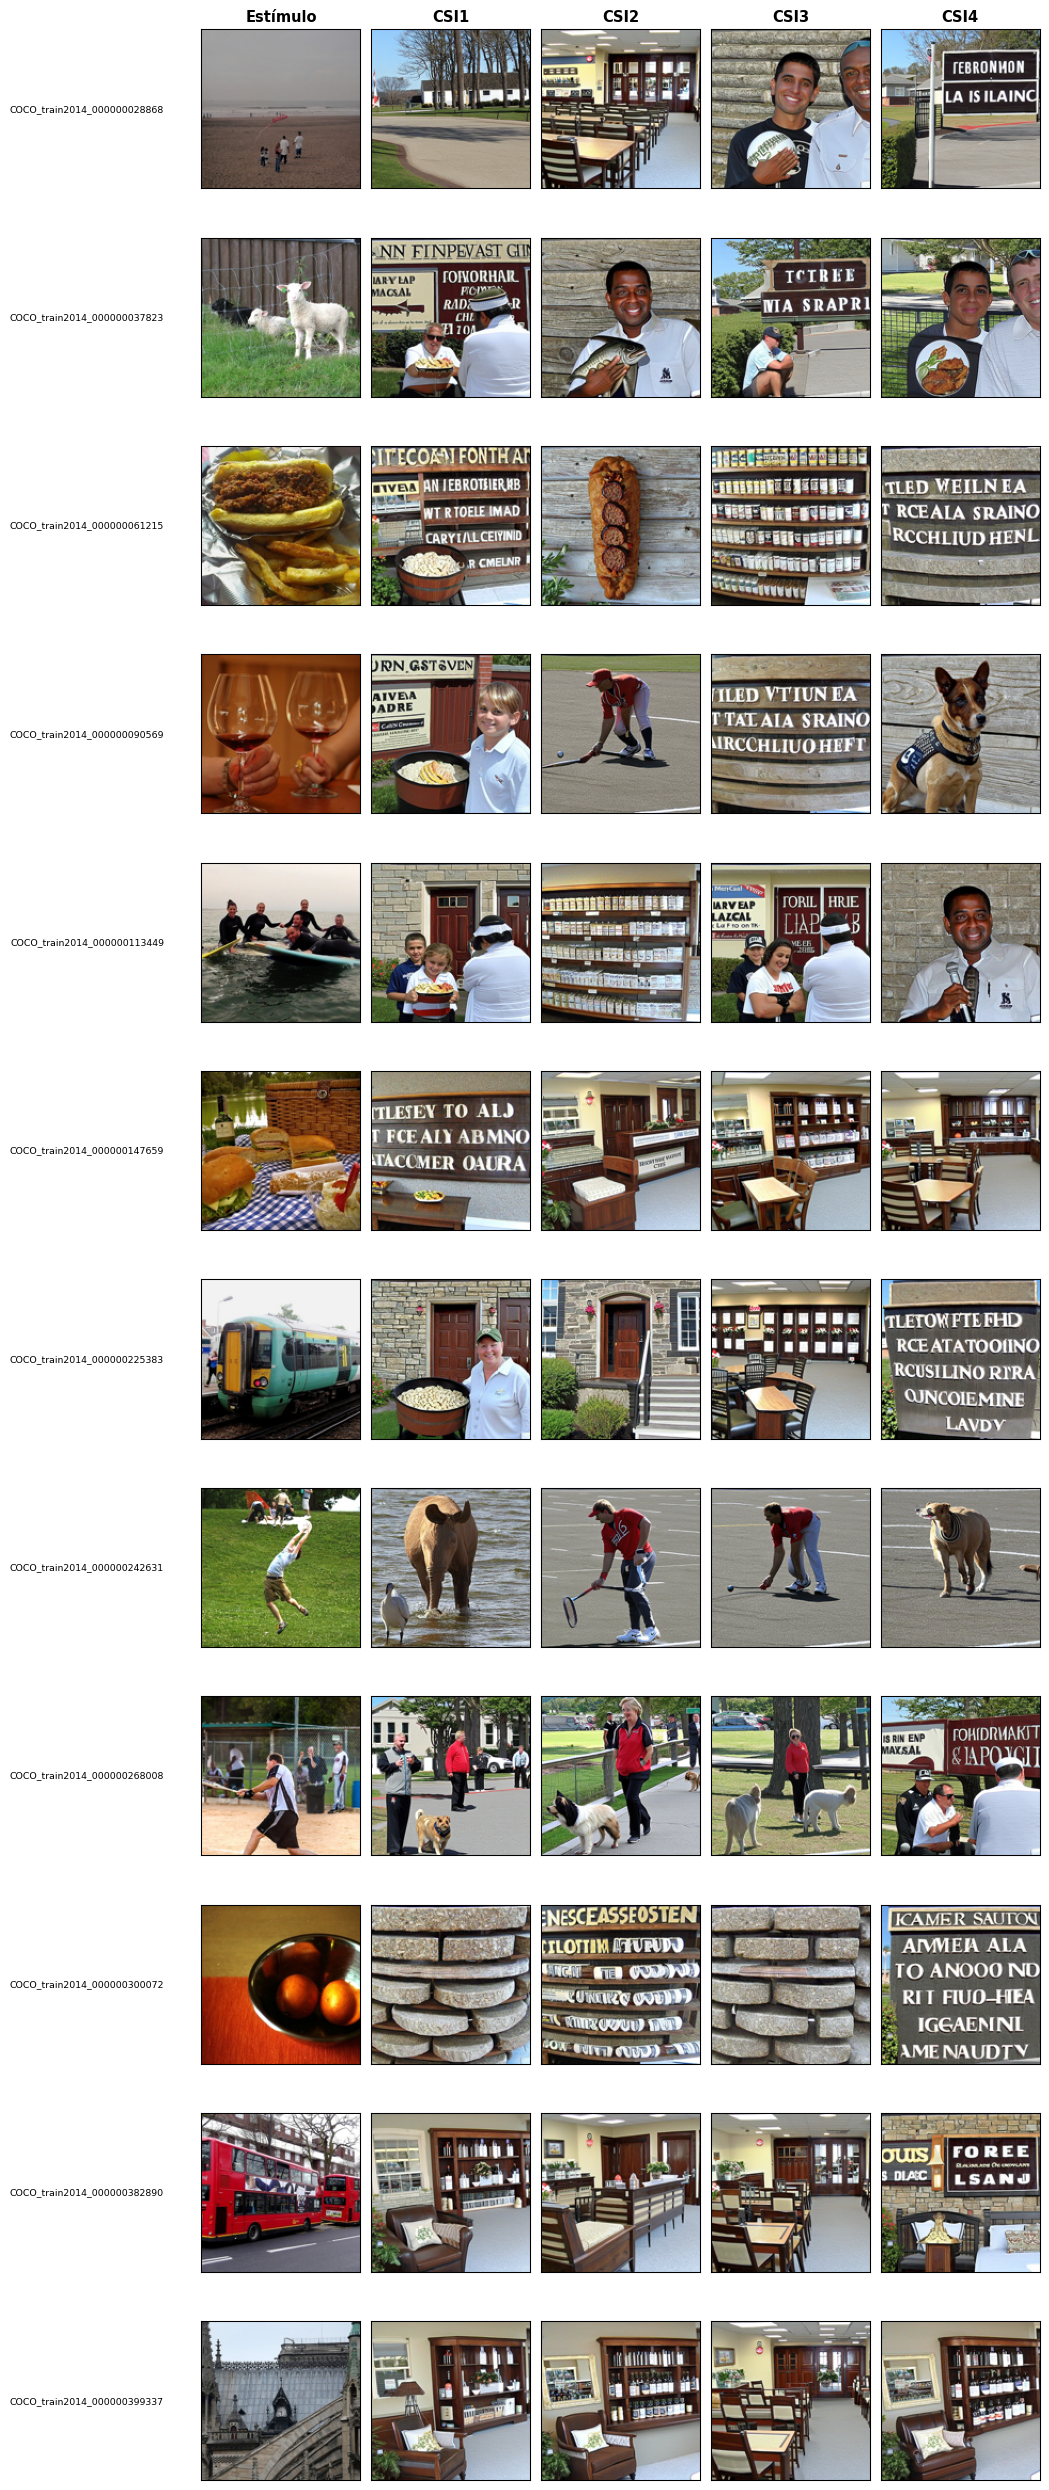
\includegraphics[width=\linewidth]{Figures/reconstrucciones/apendice/apendiceB_galeria_p01.png}
  \end{minipage}  \hfill
  \begin{minipage}[t]{0.49\textwidth}
    \centering
    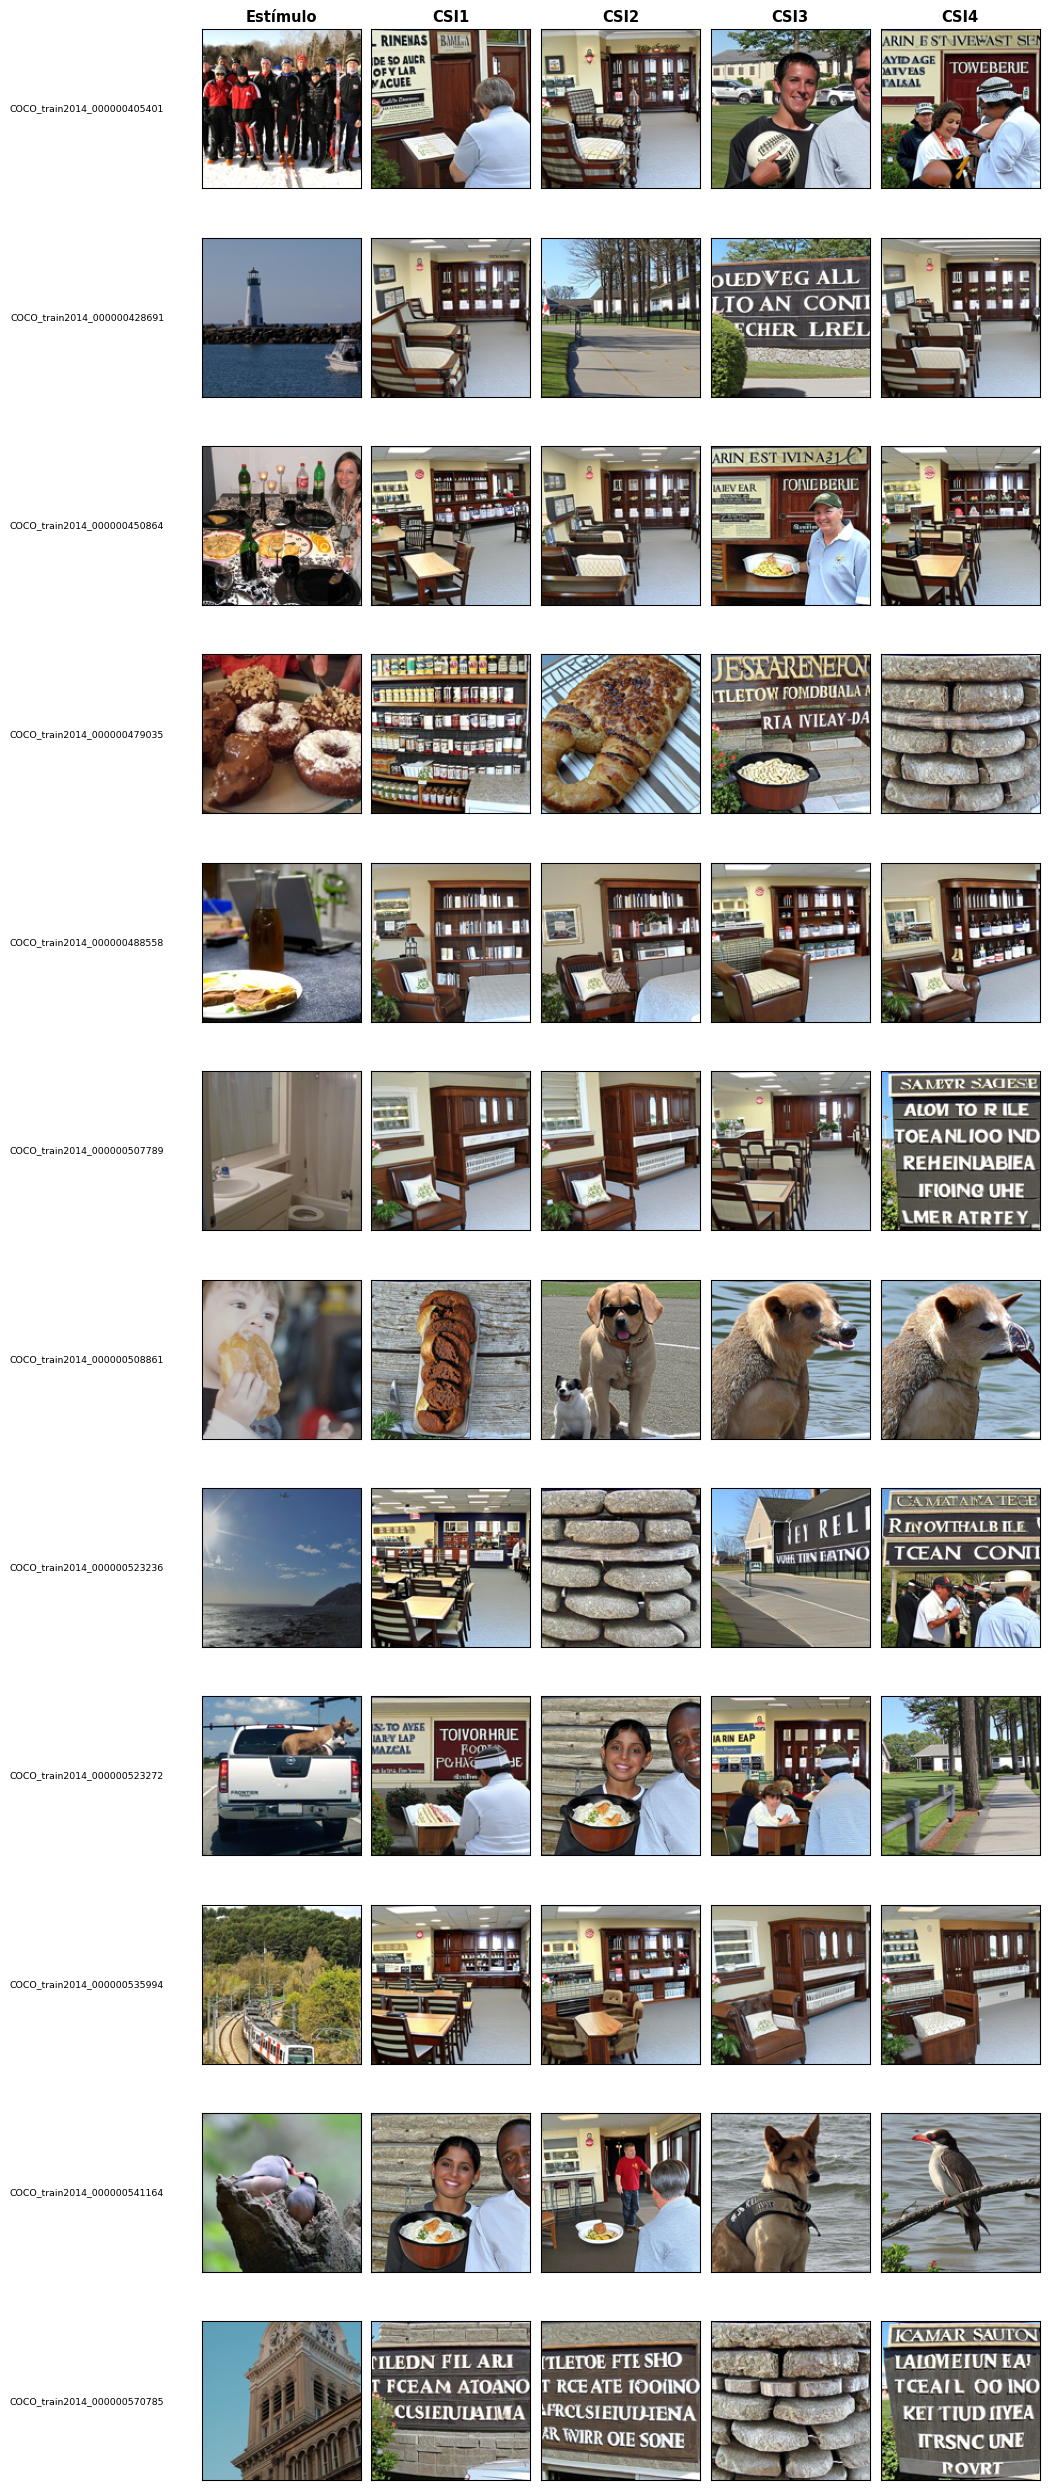
\includegraphics[width=\linewidth]{Figures/reconstrucciones/apendice/apendiceB_galeria_p02.png}
  \end{minipage}
  \caption[Galería de reconstrucciones (partes 1--2/5)]{Reconstrucciones cross-subject sobre estímulos BOLD5000 (partes 1--2 de 5). Columna~1: estímulo original; columnas~2--5: reconstrucción SD~2.1 unCLIP por sujeto (CSI1, CSI2, CSI3, CSI4).}
  \label{fig:apendiceB_galeria:g01}
\end{figure}
\clearpage

\begin{figure}[htbp]
  \centering
  \begin{minipage}[t]{0.49\textwidth}
    \centering
    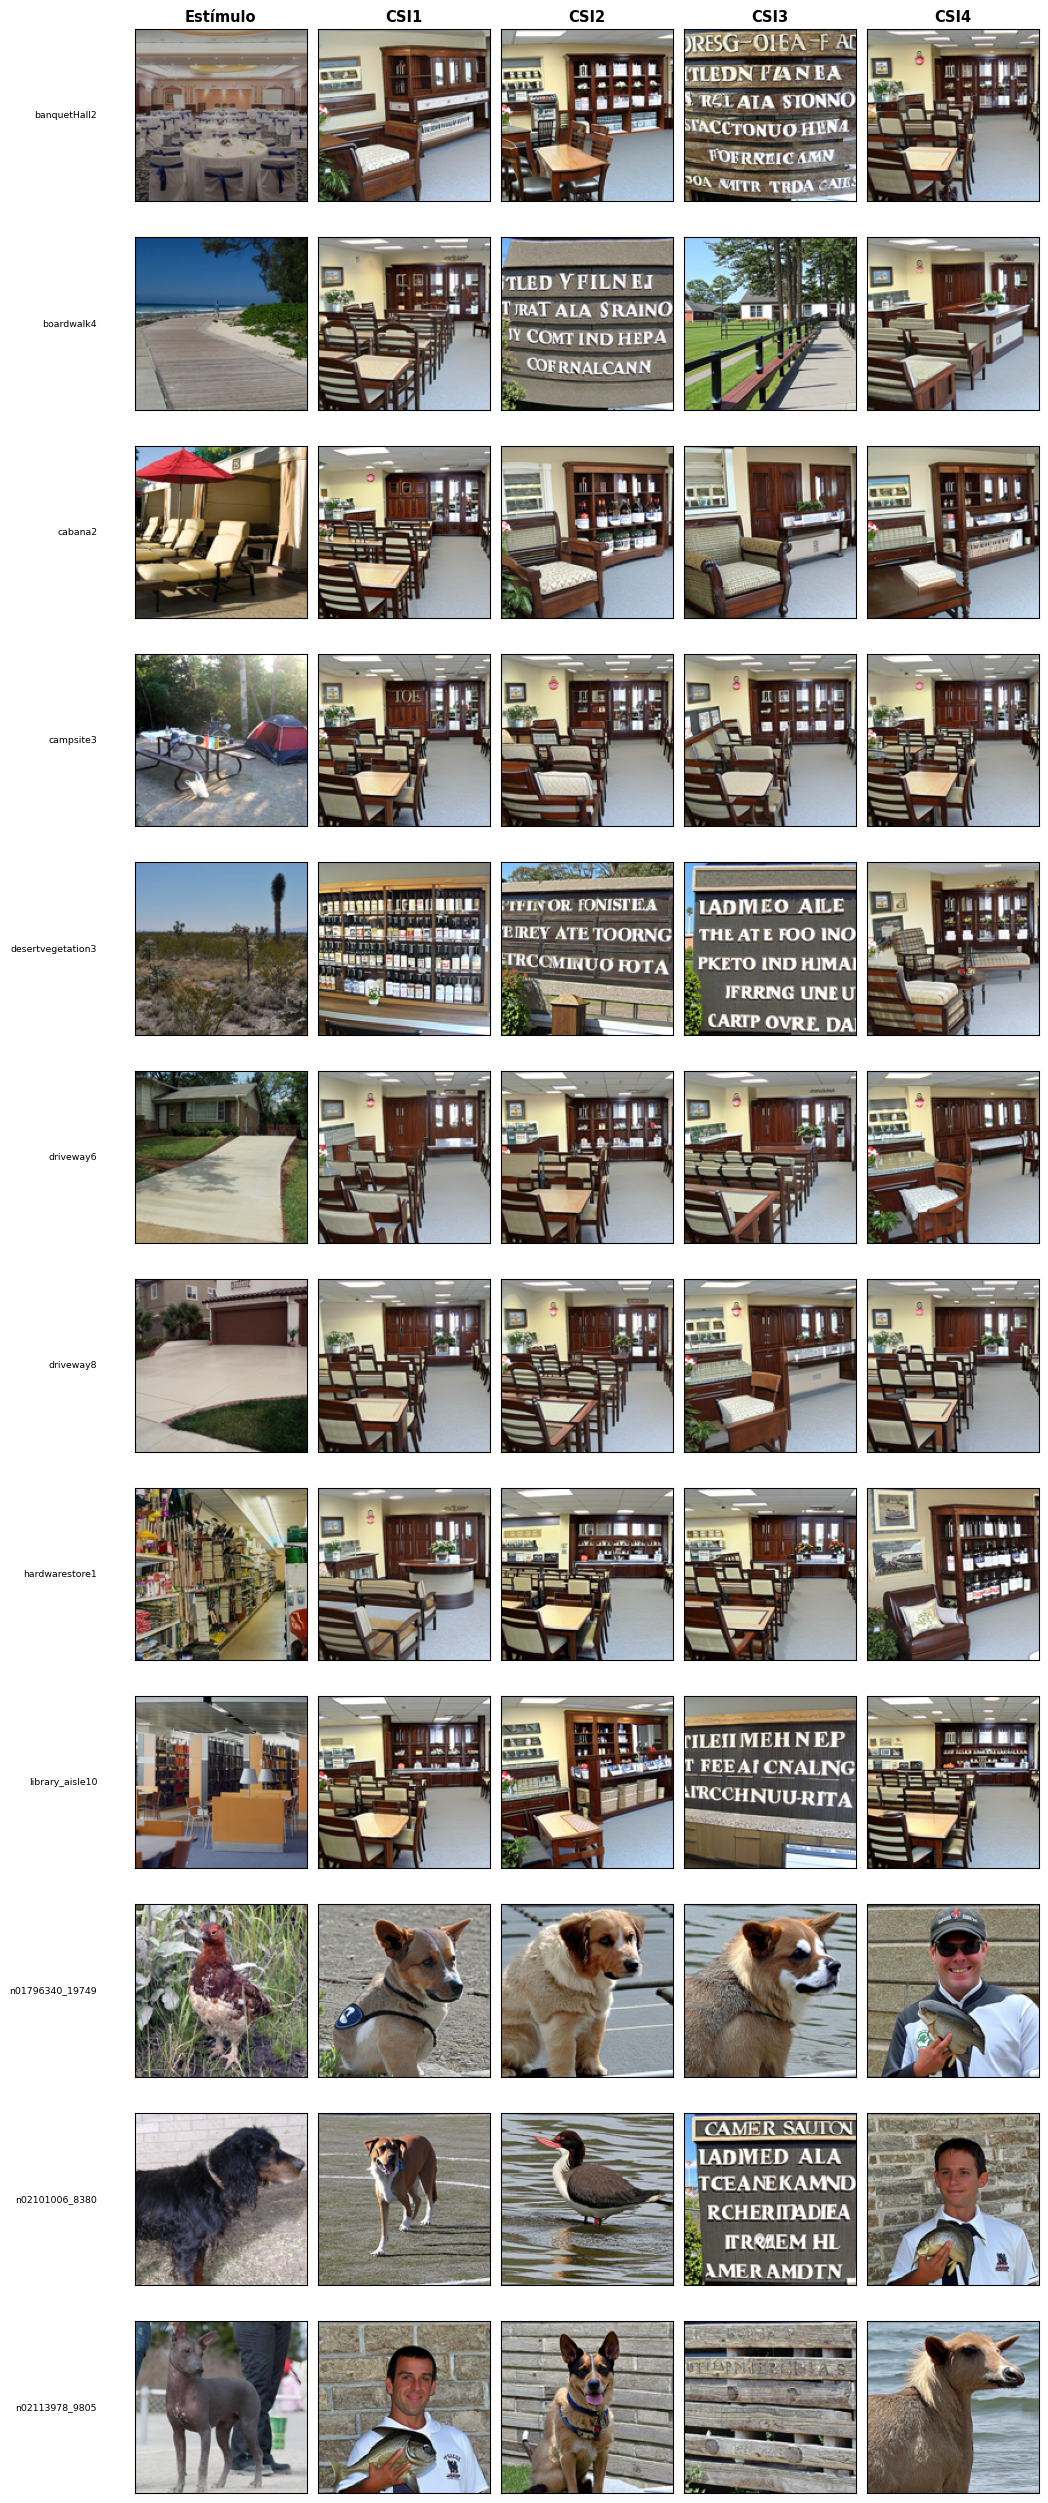
\includegraphics[width=\linewidth]{Figures/reconstrucciones/apendice/apendiceB_galeria_p03.png}
  \end{minipage}  \hfill
  \begin{minipage}[t]{0.49\textwidth}
    \centering
    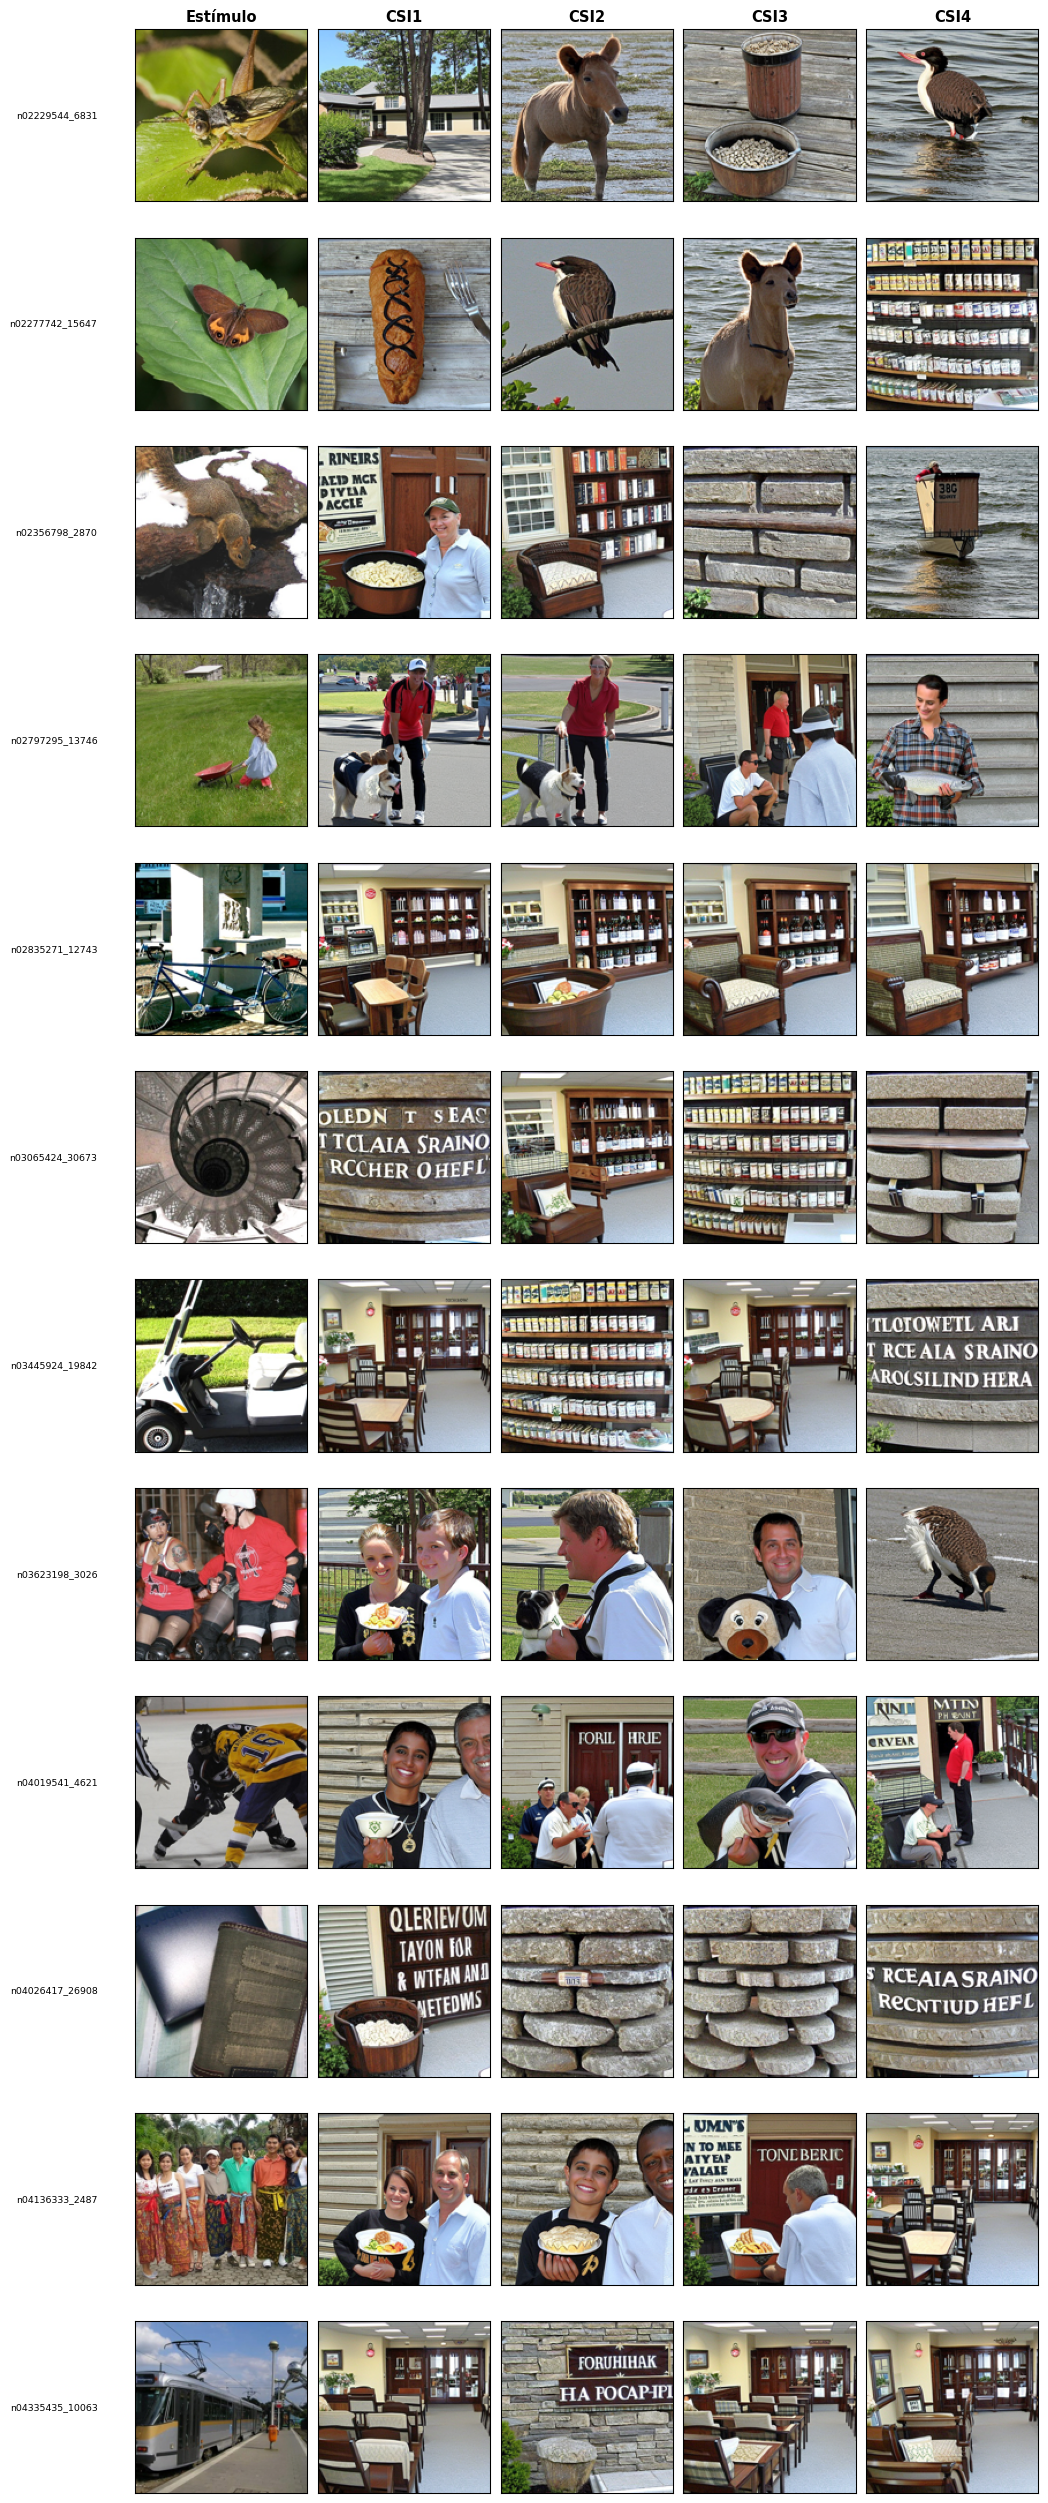
\includegraphics[width=\linewidth]{Figures/reconstrucciones/apendice/apendiceB_galeria_p04.png}
  \end{minipage}
  \caption[Galería de reconstrucciones (partes 3--4/5)]{Reconstrucciones cross-subject sobre estímulos BOLD5000 (partes 3--4 de 5). Columna~1: estímulo original; columnas~2--5: reconstrucción SD~2.1 unCLIP por sujeto (CSI1, CSI2, CSI3, CSI4).}
  \label{fig:apendiceB_galeria:g02}
\end{figure}
\clearpage

\begin{figure}[htbp]
  \centering
  \begin{minipage}[t]{0.49\textwidth}
    \centering
    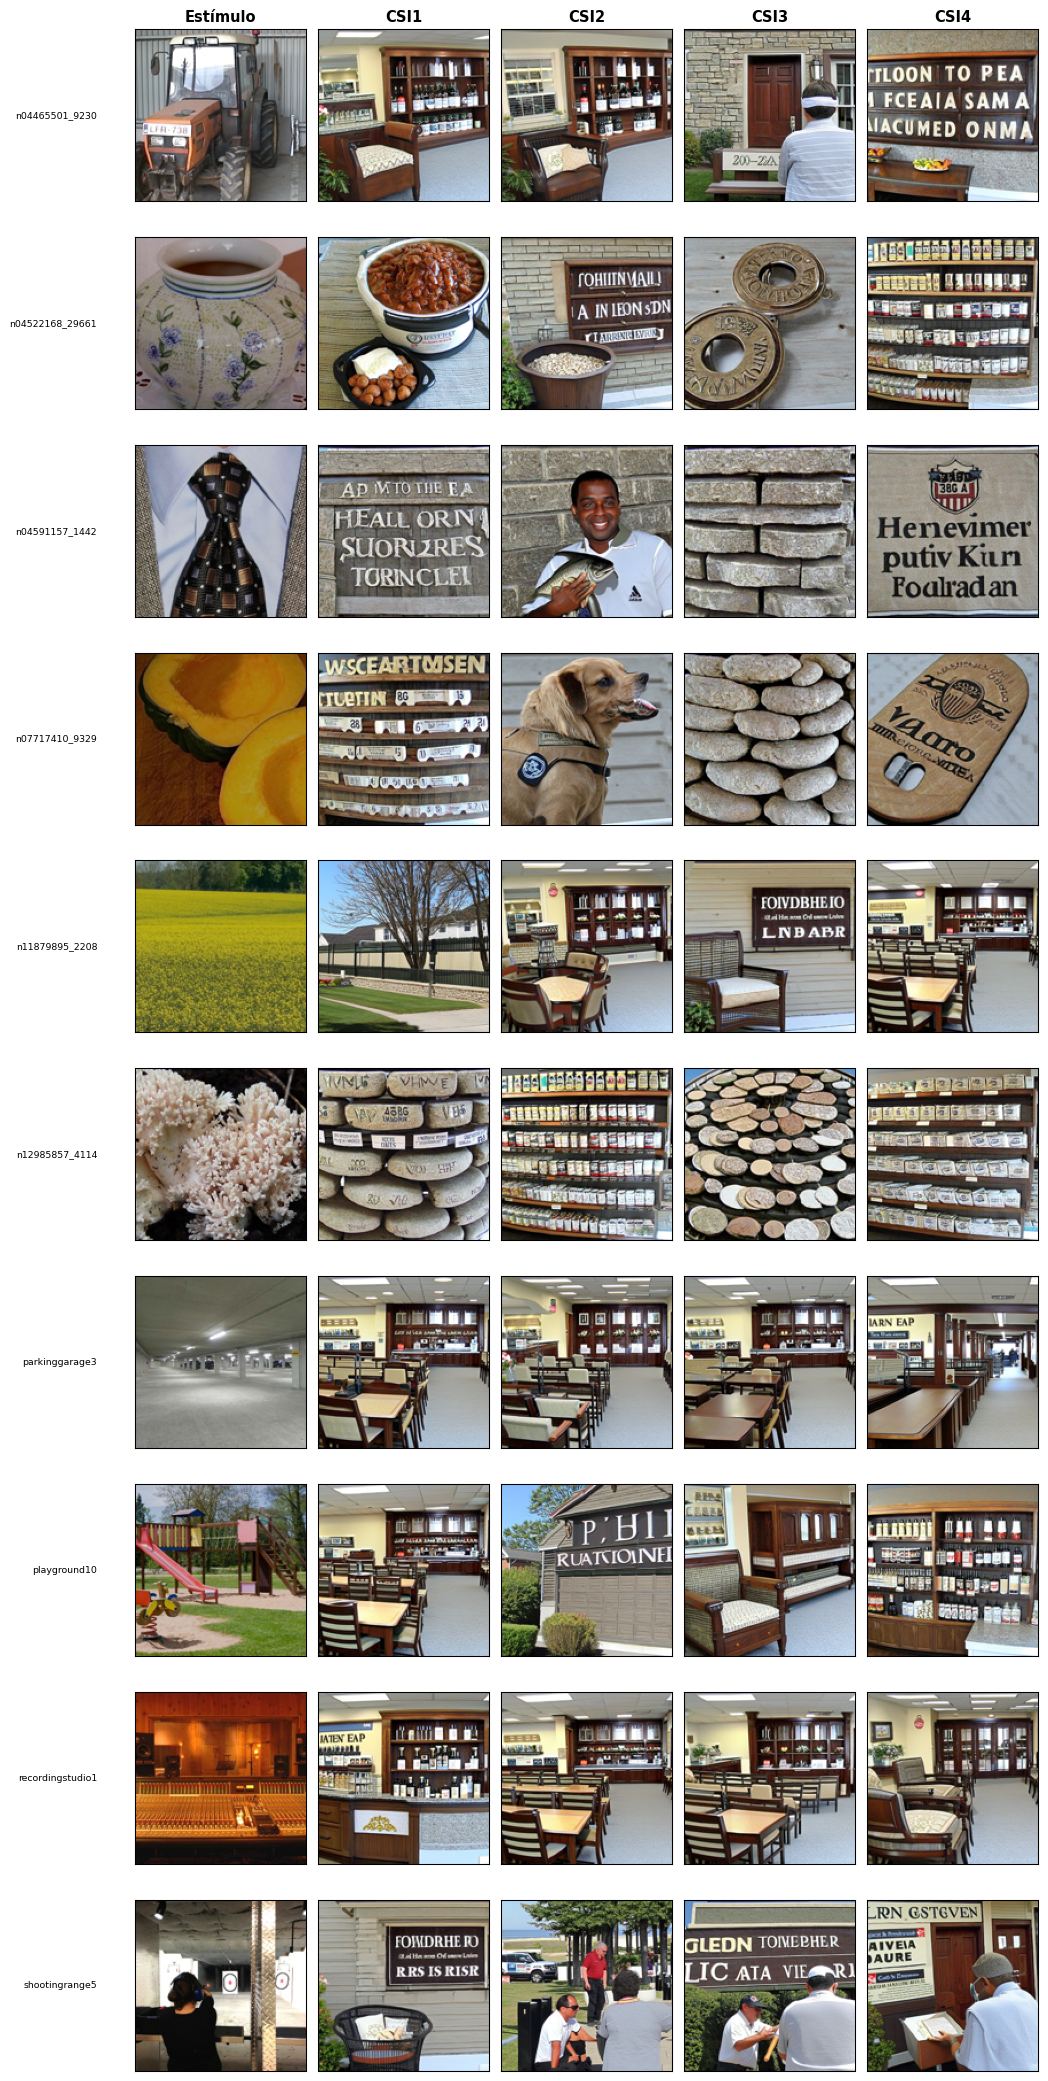
\includegraphics[width=\linewidth]{Figures/reconstrucciones/apendice/apendiceB_galeria_p05.png}
  \end{minipage}
  \caption[Galería de reconstrucciones (parte 5/5)]{Reconstrucciones cross-subject sobre estímulos BOLD5000 (parte 5 de 5). Columna~1: estímulo original; columnas~2--5: reconstrucción SD~2.1 unCLIP por sujeto (CSI1, CSI2, CSI3, CSI4).}
  \label{fig:apendiceB_galeria:g03}
\end{figure}
\clearpage
%
}{%
  \par\medskip\noindent\emph{[Galería pendiente: ejecutar
  \texttt{build\_appendix\_montages.py} y recompilar.]}\par
}

% Appendix C — Notas teóricas

\chapter{Notas teóricas}
\label{AppendC}

Este apéndice reúne las dos derivaciones que sustentan el pipeline pero que se
omitieron del cuerpo por brevedad: el modelo de difusión que genera la imagen y
la solución cerrada del regresor Ridge que mapea fMRI al espacio CLIP.

\section{Modelos de difusión: derivación abreviada}

\paragraph{Proceso directo (forward).} Un DDPM \cite{ho2020ddpm} define una
cadena de Markov que agrega ruido gaussiano a la imagen $x_0$ en $T$ pasos según
una varianza $\{\beta_t\}_{t=1}^{T}$:
\begin{equation}
  q(x_t \mid x_{t-1}) = \mathcal{N}\!\left(x_t;\, \sqrt{1-\beta_t}\,x_{t-1},\, \beta_t \mathbf{I}\right).
\end{equation}
Con $\alpha_t = 1-\beta_t$ y $\bar\alpha_t = \prod_{s=1}^{t}\alpha_s$, la
marginal admite muestreo directo en un paso:
\begin{equation}
  x_t = \sqrt{\bar\alpha_t}\,x_0 + \sqrt{1-\bar\alpha_t}\,\epsilon,\qquad \epsilon \sim \mathcal{N}(\mathbf{0},\mathbf{I}).
\end{equation}

\paragraph{Proceso inverso (reverse).} Una red $\epsilon_\theta(x_t,t)$ aprende a
predecir el ruido; el entrenamiento minimiza el objetivo simplificado
\begin{equation}
  \mathcal{L}_\text{simple} = \mathbb{E}_{x_0,\epsilon,t}\!\left[\,\bigl\|\epsilon - \epsilon_\theta(x_t,t)\bigr\|^2\,\right].
\end{equation}
El muestreo parte de $x_T \sim \mathcal{N}(\mathbf{0},\mathbf{I})$ y aplica la
media posterior estimada paso a paso hasta $x_0$.

\paragraph{Guía sin clasificador (CFG).} Para condicionar la generación por un
vector $c$ (aquí el embedding CLIP predicho desde fMRI) se combina la predicción
condicional e incondicional con una escala de guía $w$
\cite{ho2022cfg}:
\begin{equation}
  \tilde\epsilon_\theta(x_t,t,c) = (1+w)\,\epsilon_\theta(x_t,t,c) - w\,\epsilon_\theta(x_t,t,\varnothing).
\end{equation}
En este trabajo $c$ es el \emph{image embedding} CLIP ViT-L/14 y el generador es
SD~2.1 unCLIP \cite{ramesh2022unclip,rombach2022ldm}; el valor
\emph{guidance\_scale}$=8.0$ (Ap.~\ref{AppendA}) fija el compromiso entre fidelidad
al vector del cerebro y coherencia visual.

\section{Derivación de la solución cerrada de Ridge}

El adapter lineal estima $W \in \mathbb{R}^{d\times p}$ que mapea $p$ vóxeles a
las $d=768$ dimensiones del espacio CLIP. Dadas $X \in \mathbb{R}^{n\times p}$
(betas) e $Y \in \mathbb{R}^{n\times d}$ (targets CLIP), la regresión Ridge
\cite{hoerl1970ridge} minimiza el error cuadrático con penalización $\ell_2$:
\begin{equation}
  \mathcal{L}(W) = \lVert XW - Y \rVert_F^2 + \lambda \lVert W \rVert_F^2.
\end{equation}
El objetivo es convexo y diferenciable; su gradiente es
\begin{equation}
  \nabla_W \mathcal{L} = 2X^\top(XW - Y) + 2\lambda W.
\end{equation}
Igualando a cero, $X^\top X W + \lambda W = X^\top Y$, y factorizando $W$ se
obtiene la solución cerrada
\begin{equation}
  W^\star = \left(X^\top X + \lambda \mathbf{I}\right)^{-1} X^\top Y.
\end{equation}
El término $\lambda\mathbf{I}$ garantiza que la matriz sea invertible incluso con
$p > n$ (más vóxeles que trials), régimen habitual en fMRI. El \emph{shrinkage}
que introduce $\lambda$ reduce la varianza a costa de sesgar la magnitud del
embedding hacia cero; por ello \texttt{visual\_evaluator.py} ofrece el modo de
normalización \texttt{ridge}, que reescala la norma antes de inyectar el vector a
SD~2.1 unCLIP. La variante \texttt{adapter\_ridge\_stoch.py} sustituye la
inversión exacta por descenso estocástico, habilitando penalizaciones no
cerradas y constituyendo el peldaño de contribución hacia los talleres
siguientes.


\end{document}
